% !TeX encoding = UTF-8
% !TeX program = xelatex
% !TeX spellcheck = en_US

\documentclass[degree=master, degree-type=academic, language=english, fontset=mac]{thuthesis}
  % 学位 degree:
  %   doctor | master | bachelor | postdoc
  % 学位类型 degree-type:
  %   academic(默认)| professional
  % 语言 language
  %   chinese(默认)| english
  % 字体库 fontset
  %   windows | mac | fandol | ubuntu
  % 建议终版使用 Windows 平台的字体编译


% 论文基本配置,加载宏包等全局配置
% !TeX root = ./thuthesis-example.tex

% 论文基本信息配置

\thusetup{
  %******************************
  % 注意:
  %   1. 配置里面不要出现空行
  %   2. 不需要的配置信息可以删除
  %   3. 建议先阅读文档中所有关于选项的说明
  %******************************
  %
  % 输出格式
  %   选择打印版(print)或用于提交的电子版(electronic),前者会插入空白页以便直接双面打印
  %
  output = print,
  % 格式类型
  %   默认为论文(thesis),也可以设置为开题报告(proposal)
  % thesis-type = proposal,
  %
  % 标题
  %   可使用“\\”命令手动控制换行
  %
  title  = {清华大学学位论文 \LaTeX{} 模板\\使用示例文档 v\version},
  title* = {Predicting the Michaelis Constant using Sequence-based and Structure-based Methods},
  %
  % 学科门类
  %   1. 学术型
  %      - 中文
  %        需注明所属的学科门类,例如:
  %        哲学、经济学、法学、教育学、文学、历史学、理学、工学、农学、医学、
  %        军事学、管理学、艺术学
  %      - 英文
  %        博士:Doctor of Philosophy
  %        硕士:
  %          哲学、文学、历史学、法学、教育学、艺术学门类,公共管理学科
  %          填写“Master of Arts“,其它填写“Master of Science”
  %   2. 专业型
  %      直接填写专业学位的名称,例如:
  %      教育博士、工程硕士等
  %      Doctor of Education, Master of Engineering
  %   3. 本科生不需要填写
  %
  degree-category  = {工学硕士},
  degree-category* = {Master of Science},
  %
  % 培养单位
  %   填写所属院系的全名
  %
  department = {计算机科学与技术系},
  %
  % 学科
  %   1. 研究生学术型学位,获得一级学科授权的学科填写一级学科名称,其他填写二级学科名称
  %   2. 本科生填写专业名称,第二学位论文需标注“(第二学位)”
  %
  discipline  = {计算机科学与技术},
  discipline* = {Computer Science and Technology},
  %
  % 专业领域
  %   1. 设置专业领域的专业学位类别,填写相应专业领域名称
  %   2. 2019 级及之前工程硕士学位论文,在 `engineering-field` 填写相应工程领域名称
  %   3. 其他专业学位类别的学位论文无需此信息
  %
  % professional-field  = {计算机技术},
  % professional-field* = {Computer Technology},
  %
  % 姓名
  %
  author  = {Raphael Perri},
  author* = {Raphael Perri},
  %
  % 指导教师
  %   中文姓名和职称之间以英文逗号“,”分开,下同
  %
  supervisor  = {Ting Chen},
  supervisor* = {Professor Ting Chen},
  %
  % 副指导教师
  %
  % associate-supervisor  = {Jinbo Xu},
  % associate-supervisor* = {Professor Jinbo Xu},
  %
  % 联合指导教师
  %
  co-supervisor  = {Jinbo Xu, Xinyu Hong},
  co-supervisor* = {Professor Jinbo Xu, Doctor Xinyu Hong},
  %
  % 日期
  %   使用 ISO 格式;默认为当前时间
  %
  date = {2023-03-07},
  %
  % 是否在中文封面后的空白页生成书脊(默认 false)
  %
  include-spine = false,
  %
  % 密级和年限
  %   秘密, 机密, 绝密
  %
  % secret-level = {秘密},
  % secret-year  = {10},
  %
  % 博士后专有部分
  %
  % clc                = {分类号},
  % udc                = {UDC},
  % id                 = {编号},
  % discipline-level-1 = {计算机科学与技术},  % 流动站(一级学科)名称
  % discipline-level-2 = {系统结构},          % 专业(二级学科)名称
  % start-date         = {2011-07-01},        % 研究工作起始时间
}

% 载入所需的宏包

% 定理类环境宏包
\usepackage{amsthm}
% 也可以使用 ntheorem
% \usepackage[amsmath,thmmarks,hyperref]{ntheorem}

\thusetup{
  %
  % 数学字体
  % math-style = GB,  % GB | ISO | TeX
  math-font  = xits,  % stix | xits | libertinus
}

% 可以使用 nomencl 生成符号和缩略语说明
% \usepackage{nomencl}
% \makenomenclature

% 表格加脚注
\usepackage{threeparttable}

% 表格中支持跨行
\usepackage{multirow}

% 固定宽度的表格。
% \usepackage{tabularx}

% 跨页表格
\usepackage{longtable}

% 算法
\usepackage{algorithm}
\usepackage{algorithmic}

% 量和单位
\usepackage{siunitx}

% 参考文献使用 BibTeX + natbib 宏包
% 顺序编码制
\usepackage[sort]{natbib}
\bibliographystyle{thuthesis-numeric}

% 著者-出版年制
% \usepackage{natbib}
% \bibliographystyle{thuthesis-author-year}

% 本科生参考文献的著录格式
% \usepackage[sort]{natbib}
% \bibliographystyle{thuthesis-bachelor}

% 参考文献使用 BibLaTeX 宏包
% \usepackage[style=thuthesis-numeric]{biblatex}
% \usepackage[style=thuthesis-author-year]{biblatex}
% \usepackage[style=gb7714-2015]{biblatex}
% \usepackage[style=apa]{biblatex}
% \usepackage[style=mla-new]{biblatex}
% 声明 BibLaTeX 的数据库
% \addbibresource{ref/refs.bib}

% 定义所有的图片文件在 figures 子目录下
\graphicspath{{figures/}}

% 数学命令
\makeatletter
\newcommand\dif{%  % 微分符号
  \mathop{}\!%
  \ifthu@math@style@TeX
    d%
  \else
    \mathrm{d}%
  \fi
}
\makeatother

% hyperref 宏包在最后调用
\usepackage{hyperref}



\begin{document}

% 封面
\maketitle

% 学位论文指导小组、公开评阅人和答辩委员会名单
% 本科生不需要
\input{data/committee}

% 使用授权的说明
% 本科生开题报告不需要
\copyrightpage
% 将签字扫描后授权文件 scan-copyright.pdf 替换原始页面
% \copyrightpage[file=scan-copyright.pdf]

\frontmatter
% !TeX root = ../thuthesis-example.tex

% 中英文摘要和关键字

\begin{abstract}
  论文的摘要是对论文研究内容和成果的高度概括。
  摘要应对论文所研究的问题及其研究目的进行描述,对研究方法和过程进行简单介绍,对研究成果和所得结论进行概括。
  摘要应具有独立性和自明性,其内容应包含与论文全文同等量的主要信息。
  使读者即使不阅读全文,通过摘要就能了解论文的总体内容和主要成果。

  论文摘要的书写应力求精确、简明。
  切忌写成对论文书写内容进行提要的形式,尤其要避免“第 1 章……;第 2 章……;……”这种或类似的陈述方式。

  关键词是为了文献标引工作、用以表示全文主要内容信息的单词或术语。
  关键词不超过 5 个,每个关键词中间用分号分隔。

  % 关键词用“英文逗号”分隔,输出时会自动处理为正确的分隔符
  \thusetup{
    keywords = {关键词 1, 关键词 2, 关键词 3, 关键词 4, 关键词 5},
  }
\end{abstract}

\begin{abstract*}
  Enzymes are specific proteins that accelerate the rates of reactions. 
  Almost all metabolic reactions in cells need to be catalyzed in order to occur at 
  rates fast enough to substain life. Hence, understanding the mechanisms by which enzymes
  catalyze reactions is of the utmost importance not only to understand life but also to
  create new enzymes with enhance properties. A possible method is to the study the 
  Michaelis constant $K_m$, the substrate concentration at which the reaction velocity
  is 50\% of the maximum velocity. This can help measure the affinity of an enzyme with
  its substrate, the molecule it catalyze the reaction of. To do so, recent methods have
  shown promissing results using sequence-based model such as large language models for
  proteins. However, structure-based methods have not been extensively research. In this
  work, we evaluate both methods and build a combined model using both the sequence and 
  the structure information to predict the Michaelis constant. Our model outperforms
  the state-of-the-art methods for completely unseen proteins and substrates. This model
  can then be used as a scoring model to evaluate newly design pr

  % Use comma as separator when inputting
  \thusetup{
    keywords* = {keyword 1, keyword 2, keyword 3, keyword 4, keyword 5},
  }
\end{abstract*}


% 目录
\tableofcontents

% 插图和附表清单
% 本科生的插图索引和表格索引需要移至正文之后、参考文献前
% \listoffiguresandtables  % 插图和附表清单(仅限研究生)
\listoffigures           % 插图清单
\listoftables            % 附表清单

% 符号对照表
% !TeX root = ../thuthesis-example.tex

\begin{denotation}[3cm]
  \item[NLP] Natural Language Processing
  \item[LLM] Large Language Model
  \item[LPM] Large Protein Model
  \item[GNN] Graph-Neural Network
  \item[CNN] Convolutional Neural Network
  \item[GAN] Generative Adversarial Network
  \item[VAE] Variational Autoencoders
  \item[QSAR] Quantitative Structure-Activity Relationships
  \item[EC] Enzyme Commission
  \item[SMILES] Simplified Molecular Input Line Entry System
  \item[UniProt] Universal Protein Resource
  \item[PDB] Protein Data Bank
\end{denotation}



% 也可以使用 nomencl 宏包,需要在导言区
% \usepackage{nomencl}
% \makenomenclature

% 在这里输出符号说明
% \printnomenclature[3cm]

% 在正文中的任意为都可以标题
% \nomenclature{PI}{聚酰亚胺}
% \nomenclature{MPI}{聚酰亚胺模型化合物,N-苯基邻苯酰亚胺}
% \nomenclature{PBI}{聚苯并咪唑}
% \nomenclature{MPBI}{聚苯并咪唑模型化合物,N-苯基苯并咪唑}
% \nomenclature{PY}{聚吡咙}
% \nomenclature{PMDA-BDA}{均苯四酸二酐与联苯四胺合成的聚吡咙薄膜}
% \nomenclature{MPY}{聚吡咙模型化合物}
% \nomenclature{As-PPT}{聚苯基不对称三嗪}
% \nomenclature{MAsPPT}{聚苯基不对称三嗪单模型化合物,3,5,6-三苯基-1,2,4-三嗪}
% \nomenclature{DMAsPPT}{聚苯基不对称三嗪双模型化合物(水解实验模型化合物)}
% \nomenclature{S-PPT}{聚苯基对称三嗪}
% \nomenclature{MSPPT}{聚苯基对称三嗪模型化合物,2,4,6-三苯基-1,3,5-三嗪}
% \nomenclature{PPQ}{聚苯基喹噁啉}
% \nomenclature{MPPQ}{聚苯基喹噁啉模型化合物,3,4-二苯基苯并二嗪}
% \nomenclature{HMPI}{聚酰亚胺模型化合物的质子化产物}
% \nomenclature{HMPY}{聚吡咙模型化合物的质子化产物}
% \nomenclature{HMPBI}{聚苯并咪唑模型化合物的质子化产物}
% \nomenclature{HMAsPPT}{聚苯基不对称三嗪模型化合物的质子化产物}
% \nomenclature{HMSPPT}{聚苯基对称三嗪模型化合物的质子化产物}
% \nomenclature{HMPPQ}{聚苯基喹噁啉模型化合物的质子化产物}
% \nomenclature{PDT}{热分解温度}
% \nomenclature{HPLC}{高效液相色谱(High Performance Liquid Chromatography)}
% \nomenclature{HPCE}{高效毛细管电泳色谱(High Performance Capillary lectrophoresis)}
% \nomenclature{LC-MS}{液相色谱-质谱联用(Liquid chromatography-Mass Spectrum)}
% \nomenclature{TIC}{总离子浓度(Total Ion Content)}
% \nomenclature{\textit{ab initio}}{基于第一原理的量子化学计算方法,常称从头算法}
% \nomenclature{DFT}{密度泛函理论(Density Functional Theory)}
% \nomenclature{$E_a$}{化学反应的活化能(Activation Energy)}
% \nomenclature{ZPE}{零点振动能(Zero Vibration Energy)}
% \nomenclature{PES}{势能面(Potential Energy Surface)}
% \nomenclature{TS}{过渡态(Transition State)}
% \nomenclature{TST}{过渡态理论(Transition State Theory)}
% \nomenclature{$\increment G^\neq$}{活化自由能(Activation Free Energy)}
% \nomenclature{$\kappa$}{传输系数(Transmission Coefficient)}
% \nomenclature{IRC}{内禀反应坐标(Intrinsic Reaction Coordinates)}
% \nomenclature{$\nu_i$}{虚频(Imaginary Frequency)}
% \nomenclature{ONIOM}{分层算法(Our own N-layered Integrated molecular Orbital and molecular Mechanics)}
% \nomenclature{SCF}{自洽场(Self-Consistent Field)}
% \nomenclature{SCRF}{自洽反应场(Self-Consistent Reaction Field)}



% 正文部分
\mainmatter
% !TeX root = ../thuthesis-example.tex

\chapter{Introduction}
\label{chap:1}

Enzymes are proteins that catalyze biological reactions. They accelerate reactions 
to a speed that supports metabolic processes necessary for life. 
Understanding how enzymes work is crucial not only for grasping fundamental 
biological mechanisms but also for advancing medical science, 
particularly in the development of new pharmaceuticals and the engineering 
of enzymes with enhanced properties.

In order to design effective drugs or improve enzyme functions, 
one major challenge is the selection of the most promising compounds 
from a vast array of possibilities. 
Laboratory testing is costly and time-consuming. To reduce the possibilities,
using kinetic information can become a promising solution.

A key parameter in enzyme kinetics is the Michaelis constant ($K_m$). It represents
the substrate concentration at which the initial velocity of the reaction is half of
the maximum velocity. Generally, the lower the value, the higher is the affinity 
between the enzyme and the substrate.

Therefore, predicting the Michaelis constant can significantly accelerate the drug design process. 
By estimating an enzyme's affinity for various substrates and similarly, several enzymes
with one substrate, researchers can prioritize compounds for further development, 
thereby reducing the need for extensive laboratory testing. 
This approach not only facilitates the discovery of new drugs but also enhances 
our ability to engineer enzymes with desired characteristics.

\section{Problem statement}

The goal of this work is to build a statistical regression model that predict the 
Michaelis constant given 2 inputs: the protein sequence and the substrate string. 

The performance of the model will be evaluated with the mean squared error (MSE) and 
the coefficient of determination $r^2$.

\section{Literature review}

Given the interdisciplinary nature of this thesis, which involves biological, chemical, and 
computer sciences, the literature review will be structured in the following way.

First, the reader will be provided with the biological and chemical fundamentals necesarry to understand basic aspects
of enzyme kinetics. This foundation is essential to comprehend the biological processes at play and
their relevance to our work.

Second, machine learning and deep learning methodologies, emphasizing on their biological
applications, will be presented. This section aims to present how statistical models can be used to decipher complex biological
data, hence allowing us to build innovative solutions in enzyme and drug design.

Finally, a specific focus on the current state of research regarding the prediction of the Michaelis 
constant ($K_m$) will be offered. The aim of this part is to highlight the current contributions to 
our problem statement, the current state-of-the-art methods used, and their results.

Through this comprehensive review,the solid background provided will ensure the relevance of this thesis
contribution in the field of drug design.

\subsection{Biological and Chemistry Background}
\subsubsection{Proteins}
Proteins impact all the processes that take place in a cell, with an almost
endless diversity of functions. They are the most abundant biological macromolecules.
Thousands of different types of proteins can be found in a single cell. They are the molecular
instruments through which genetic information is expressed.\cite{lehninger}.

A protein is a sequence of smaller molecules called amino acids that are covalently joined by a peptide
bond. There exists 20 common amino acids (Figure \ref{fig:20aa}) from which almost all proteins are made of. Each amino acid has
a side chain with distinctive chemical properties.

\begin{figure}
  \centering
  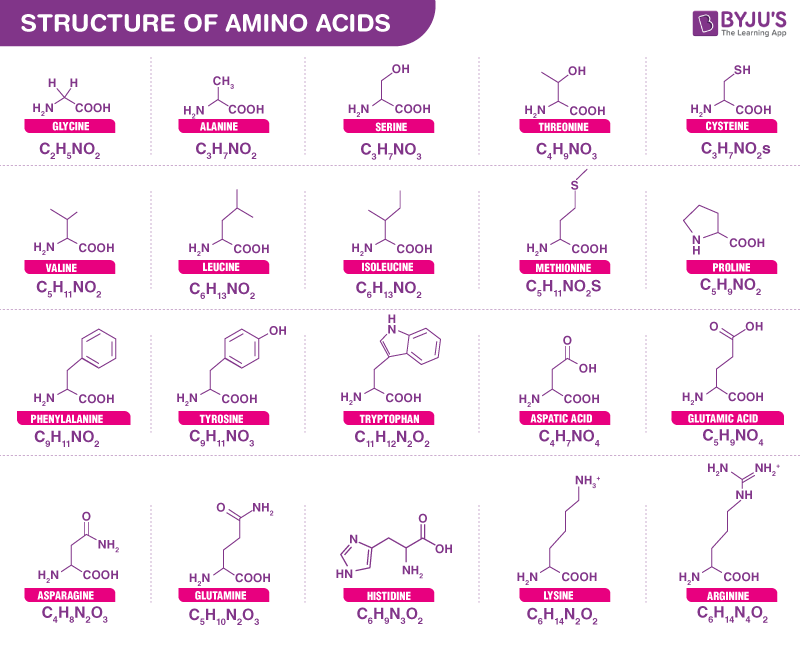
\includegraphics[width=0.7\linewidth]{1-amino_acids.png}
  \caption{The 20 common amino acids}
  % https://www.google.com.hk/url?sa=i&url=https%3A%2F%2Fbyjus.com%2Fbiology%2Famino-acids%2F&psig=AOvVaw1r9URV_-jl8bxr1TZ5ehjk&ust=1710296952635000&source=images&cd=vfe&opi=89978449&ved=0CBMQjRxqFwoTCIjpnuXW7YQDFQAAAAAdAAAAABAE
  \label{fig:20aa}
\end{figure}

All common amino acids are $\alpha$-amino acids. This means that both the carboxyl group and the amino group
is bonded to the same carbon atom called the $\alpha$-carbon (Figure \ref{fig:aastructure}). The amino acids differ from each others in
their side chains, also called R-groups, which vary in size, structure, electronic charge, and which
influence the solubility of the amino acids in water.

\begin{figure}
  \centering
  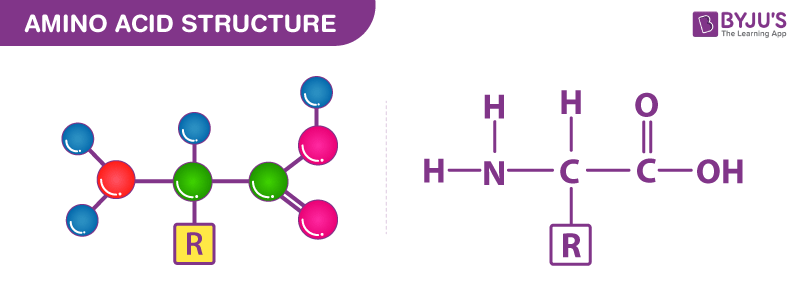
\includegraphics[width=0.3\linewidth]{1-amino_acid_structure.png}
  \caption{Amino acid structure}
  % https://www.google.com.hk/url?sa=i&url=https%3A%2F%2Fen.wikipedia.org%2Fwiki%2FAmino_acid&psig=AOvVaw1uUyMqtMb_u6DnLzN1XZTr&ust=1710297308181000&source=images&cd=vfe&opi=89978449&ved=0CBMQjRxqFwoTCOiroY7Y7YQDFQAAAAAdAAAAABAD
  \label{fig:aastructure}
\end{figure}

Two amino acids can be joined together with a covalent bond that is called a peptide bond. This link
is formed by the removal of the element of water (a hydroxyl group from the $\alpha$-carboxyl group
of one amino acid and a hydrogen atom from the $\alpha$-amino group of another amino acid. Figure 
\ref{fig:peptidebond}). These joined amino acids are called residues, relfecting the loss of the element
of water during the bonding formation.

\begin{figure}
  \centering
  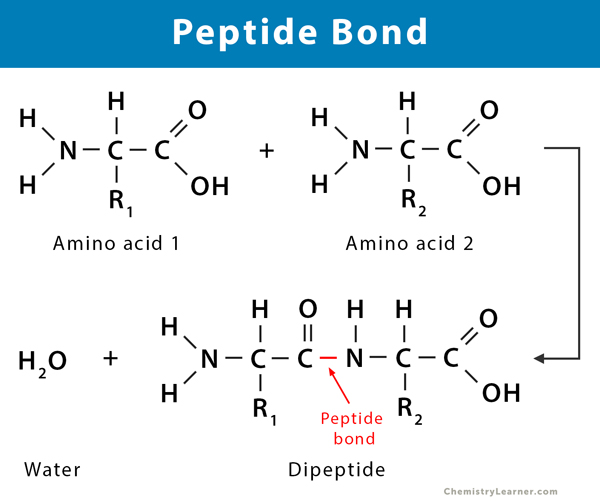
\includegraphics[width=0.5\linewidth]{1-peptide_bond.jpeg}
  \caption{Peptide bond}
  %https://www.chemistrylearner.com/wp-content/uploads/2020/10/Peptide-Bond.jpg
  \label{fig:peptidebond}
\end{figure}

An oligopeptide is the structure of a few amino acids joined together and a polypeptide is the name
given to the structure when many amino acids are joined. Proteins may have thousands of amino acids residues.

For proteins, the amino acid residues at the end are the $\alpha$-amino group called N-terminal and 
the $\alpha$-carboxyl group called C-terminal. The N-terminal is conventionally placed on the left while
the C-terminal is placed on the right.

The functions of proteins do not depend on their length or molecular weight. Some very small proteins 
(2 to 10 amino acids) can be extremely important such as toxic mushroom poisons or antibiotics (example + ref). The
length of proteins can vary enourmously from 2 to 27,000 amino acids, while the vast majority of proteins
usually contain fewer than 2,000 amino acids.

Some proteins are made of only one polypeptide chain while other can be made out of several, they are 
called mutlisubunit proteins, such as hemoglobin (example + ref).

Some proteins also contain chemical groups other than amino acids. They are called conjugated proteins.
The non-amino acid part of these proteins is called its prosthetic group and is essential to the protein
overall functions, such as hemoglobin and its ferrous group without which it does not function properly 
(check this + example + ref)

\subsubsection{Enzymes}
Enzymes are specific proteins that accelerate the rate of reactions. They are essential to life as many
of the chemical reactions essential to our survival need to be accelerated, such as the conversion of sugar.
(add example). 

\subsubsection{Pocket detection}
xxxx


\subsubsection{Substrates}
Substrates are the small molecules that interact with enzymes.

xxx
\subsubsection{Enzyme Kinetics}
kcat and Km

\subsection{Machine and Deep Learning for Drug Discovery}
\subsubsection{Traditional approaches}
\subsubsection{Machine Learning approaches}
\subsubsection{Neural Networks}
\subsubsection{Protein Language Models}
\subsubsection{Graph Neural Networks}

\subsection{Michaelis constant prediction}

Predicting the Michaelis constant represents a critical intersection of computational biology 
and enzymology, where the precise quantification of enzyme-substrate affinity becomes possible 
through advanced computational models. This section delves into the pivotal aspects of $K_m$
prediction, comprising the datasets used for model training and validation, 
the methodologies currently in practice, and an overview of the state-of-the-art performances achieved 
in this domain. 
\subsubsection{Dataset}
\label{sec:dataset}
The foundation of any computational approach to predicting the Michaelis constant is the dataset. 
This section describes the characteristics of the datasets employed, including the source of the 
protein and substrate sequences, the diversity of the enzyme classes represented, and the annotations of 
the Michaelis constant.

Before detailing the dataset preprocessing, it is essential to mention the elements it will be composed of.
The dataset will be made of 3 elements: protein sequences, a substrate string in SMILES format, and a
numerical $K_m$ value.

The SMILES (Simplified Molecular Input Line Entry System) notation is widely used method for 
representing the structure of chemical molecules using short ASCII strings. \cite{smiles}
Developed in the 1980s by Arthur Weininger and colleagues, SMILES has become a standard for the 
electronic storage of molecular information in databases and for the exchange of molecular structures 
between different software applications. It's particularly valued for its simplicity and the 
compactness of its representations, which allow for efficient processing and analysis of chemical 
structures by computers.

The key features of the SMILES notations are:
\begin{itemize}
  \item Atoms: Atoms are represented by their chemical symbol with hydrogen atoms usually 
  omitted (assumed implicitly). For example, the SMILES for ethanol (C2H5OH) is simply CCO, 
  implicitly understood as C2H6O.
  \item Bonds: Single bonds are not explicitly represented, while double, triple, 
  and aromatic bonds are denoted by =, \#, and :, respectively. For example, ethene (C2H4) 
  has the SMILES C=C.
  \item Branching: Branches are denoted by parentheses. For instance, isobutane (C4H10) can be 
  represented as CC(C)C.
  \item Rings: Ring structures are indicated by using numerical digits to represent the 
  connection point in a ring closure. For example, cyclohexane is represented as C1CCCCC1.
  \item Chirality: Chirality is specified using @ symbols. The @ symbol indicates one stereoisomer, 
  and @@ indicates the other.
\end{itemize}

Two databases using this notation are worth mentioning for to better understand the creation of the dataset:
KEGG and PubChem. \cite{kegg,pubmec} The Kyoto Encyclopedia of Genes and Genomes (KEGG) is a 
comprehensive database integrating genomic, chemical, and systemic functional information. 
It offers resources for the systematic analysis of gene functions in terms of the networks of 
genes and molecules. KEGG facilitates understanding of biological processes and their underlying 
mechanisms by categorizing gene products into their respective pathways and modules, providing a 
platform for both bioinformatics and systems biology. It possesses a unique way to identify all molecular
compounds called KEGG ID.
PubChem, on the other hand, is a database of chemical molecules and their activities 
against biological assays. Operated by the National Center for Biotechnology Information (NCBI), 
it is a vital resource for chemists, biochemists, and biologists. 
PubChem contains information on the chemical structure, identification, biological activities, 
patents, and literature citations of compounds. It supports the search for chemical substances 
by name, molecular formula, structure, and other identifiers, making it an invaluable tool for 
researchers in drug discovery and pharmacology. It also possesses a unique way to identify all molecular
compounds called PubChem ID.

The dataset used is obtained from \citeauthor{km1} as it is the standard dataset used for the most recent Michaelis
constant prediction models. It is comprised of 11,675 enzyme-substrate pairs and their associated $K_m$ value in
the format defined above: protein sequences, substrate strings in SMILES format, and numerical $K_m$ values
that have been log10 transform as the Michaelis constant values usually range from $10^{-1}$ to  $10^{-7}$.

The 11,675 entries of the dataset were compiled from the BRENDA database. \cite{brenda} The BRENDA 
(BRaunschweig ENzyme DAtabase) database is a comprehensive collection of 
enzyme and metabolic information, widely recognized as one of the most detailed 
and user-friendly resources for enzyme data. It was initially developed at the Technical 
University of Braunschweig, Germany, and has been continuously updated and expanded since its 
inception in the 1980s. BRENDA offers an extensive range of data on enzyme function, 
classification, kinetics, and molecular properties, making it an invaluable tool for 
researchers in biochemistry, molecular biology, and related fields.

At the time of the dataset creation, 156,387 entries detailing $K_m$ values, organism and substrate names, 
EC numbers, UniProt IDs of enzymes, and PubMed IDs. To enhance data specificity and compatibility, 
substrate names were aligned with KEGG Compound IDs using KEGG and PubChem synonym lists. \cite{kegg}
When necessary, PubChem IDs were mapped to KEGG IDs via MBROLE's web service. \cite{pubchem,mbrole}
Amino acid sequences were acquired through UniProt's mapping service if they were available. \cite{uniprot}
When the UniProt ID was not available, the sequence was directly retrived from BRENDA by selecting a
sequence with the same EC Number and organism. The dataset was then processed to eliminate duplicates, 
non-wild-type enzymes, 
entries from nonbacterial organisms lacking UniProt IDs, and substrates unidentifiable with KEGG IDs, 
adding up to 34,526 entries. Only entries with natural substrates were keep, 
as indicated by their presence in the KEGG reaction database, resulting in 11,675 viable data points. 
These entries were log10-transformed for consistency, with the dataset randomly divided into training 
(70\%), validation (10\%), and test (20\%) sets. 

This dataset is the most commonly used for Michaelis constant prediction. 

\subsubsection{Current Methods}

As of today, 4 models offer the best performances for predicting the Michaelis constant on the dataset
at hand. In this section, we delve into each of them.

The first model we will discuss is by the authors of the dataset themselves, \citeauthor{km1} as they were
the frist one to curate a dataset for this task and built a model for it. They offer a method using both
Machine and Deep Learning. For the substrate, it is represented as a molecular graph based on its atoms and
bonds. This information can be extracted from the SMILES representation using RDKit. \cite{rdkit} They are
then processed by a Graph Convolutional Neural Network to produce an embedding for each substrate. This 
embedding is then concatenated to a UniRep embedding of the protein sequence. \cite{unirep} 
Then, this new vector is fed into a gradient boosting model, XGBoost. \cite{xgboost}

Another model called ENKIE (ENzyme KInetics Estimator) uses hierarchical Bayesian Multilevel
Models to predict value and uncertainty of the Michaelis constant. In this paper, the assumption is that
the residuals are normally distributed, defined by means ($\mu_*$) and standard deviations ($\sigma_*$), 
accounting for the inherent variability in enzyme behavior without directly addressing 
the structural and physical complexity of the enzymes and their interactions. It categorizes data based on
substrates which introduces group-level effects that reflect the nested nature of 
biological processes. Hence, the protein sequence is not directly used but instead information about the
protein such as EC Number, protein family, and UniProt ID. Are also used reaction stoichiometries and
identifiers, as well as optionally physiological properties of the reaction compartments (pH, pMg, 
temperature and ionic strength).

\begin{figure}
  \centering
  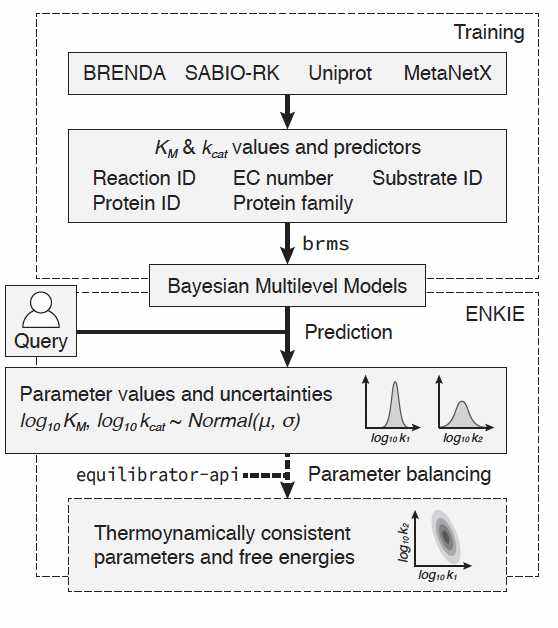
\includegraphics[width=0.5\linewidth]{1-enkie.png}
  \caption{ENKIE model overview}
  \label{fig:enkie}
\end{figure}

Published in Nature Communications, UniKP is a unified framework based on pretrained large language models
for predicting enzyme kinetic parameters: the enzyme turnover number ($k_{cat}$), the Michaelis constant
($K_m$), and the catalytic efficiency ($\frac{k_{cat}}{K_m}$). Similarly to \citeauthor{km1} is uses both the
protein sequence and the substrate string. It is comprised of 2 main components : a representation module 
for both the protein sequence (Figure \ref{fig:unikp}, part a) and the substrate string 
(Figure \ref{fig:unikp}, part b) and a machine learning module (Figure \ref{fig:unikp}, part c). 
Part d on Figure \ref{fig:unikp} are only relevent for $k_{cat}$ and include additional features into the model
such as pH and temperature. Part e of Figure \ref{fig:unikp} represents the re-weighting methods used 
to adjust the sample weight distribution to generate an optimized prediction. For the protein, the ProtT5-XL
model is used where, for each sequence, each amino acid is turned into a 1024-dimensional vector. To obtain
a condensed representation for each protein, mean pooling is applied. For the substrate, it is processed in
a similar way where each character of the string is processed by the SMILES-Transformer, resulting in a 
256-dimensional vector for each symbol. To get an equivalent 1024-dimensional vector for the substrate,
mean and max pooling are applied to these vectors and concatenated with the first and last output of the
model, as they are the start (SOS) and end of sequence (EOS). Then, both the protein and substrate representations
are contatenated and fed into the machine learning module. The latter is Extremely Randomized Trees, an
ensemble method that combines the predictions of multiple de-correlated decision trees to make more 
accurate and stable predictions than any single decision tree. It is similar to Random Forests but 
introduces extra randomness in the way splits are made at the nodes of the decision trees. \cite{extratrees}

\begin{figure}
  \centering
  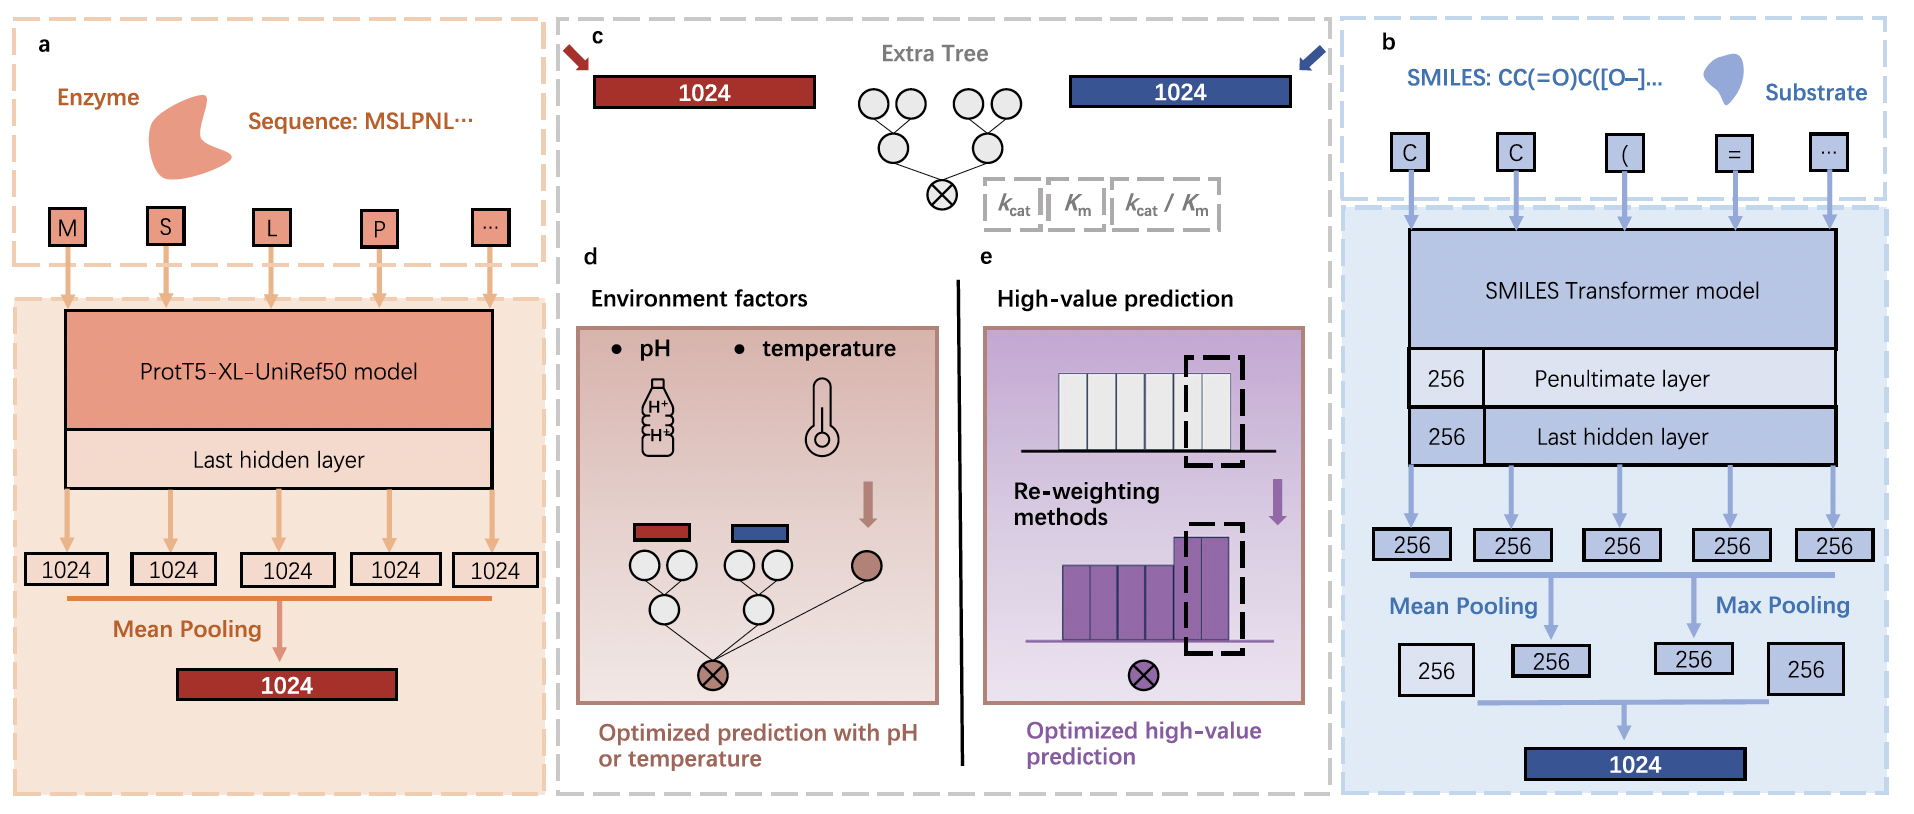
\includegraphics[width=1\linewidth]{1-unikp.png}
  \caption{UniKP model overview}
  \label{fig:unikp}
\end{figure}

Finally, the last method we will present is ProSmith. \cite{prosmith} While it hasn't been published yet
and is only available in preprint, it offers the best results for this task. This model employs a multimodal
transformer network to simultaneously process protein amino acid sequences and substrate strings. To do so,
the model use a concatenation approach where the protein sequence and substrate string are concatenated 
and separated by a separation token. In order to process this input, the network divide it into chunk 
known as tokens. For protein sequences, the tokens are the amino acids and for substrate, each symbol is
treated as a separate token. ProSmith use pre-learned token representations that were trained independently
on each modality. For amino acid representations, ESM-1b model was used and for the SMILES string tokens, it
was ChemBERTa2. \cite{esm1,chemberta} The token embeddings from ESM-1b and ChemBERTa2 have different dimensions,
1280 and 600 respectively. To process them using the same transformer network, the authors used linear layers
to map both sets of embeddings to a joint embedding space with a dimension of 768, which is also the hidden
dimension of all tokens in the ProSmith transformer network. 

\begin{figure}
  \centering
  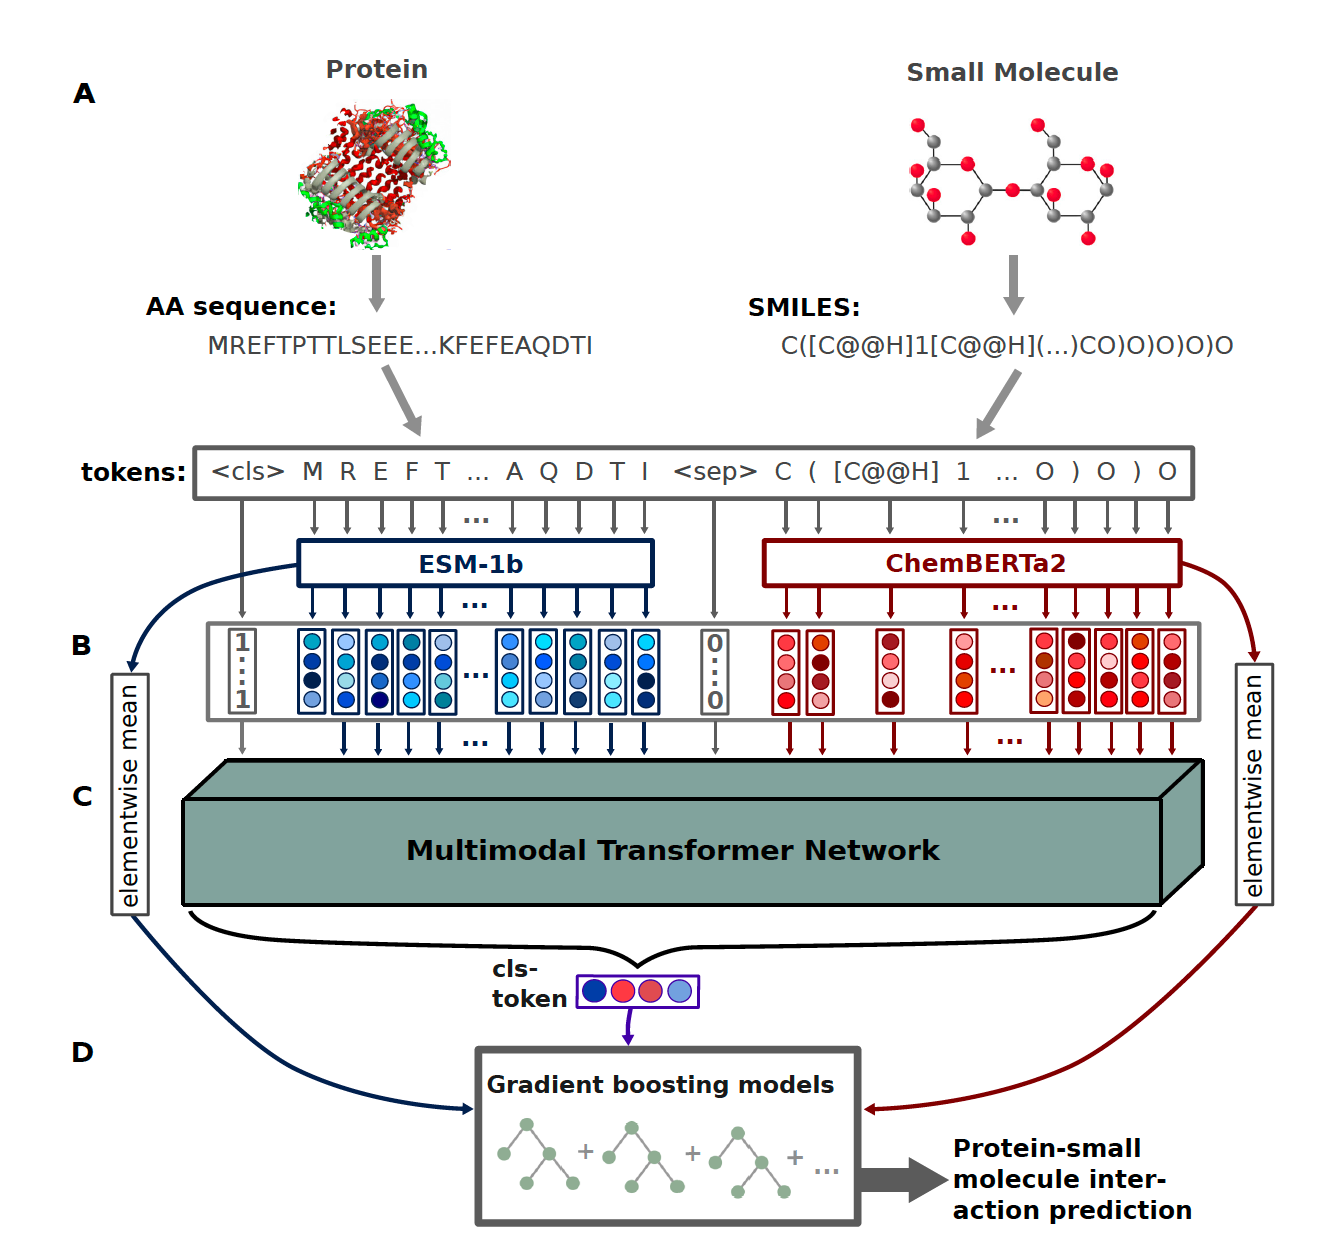
\includegraphics[width=1\linewidth]{1-prosmith.png}
  \caption{ProSmith model overview}
  \label{fig:prosmith}
\end{figure}

During the processing steps, the transformer 
network updates each input token using the attention mechanism, with 6 attention layers, each having
6 attention heads. \cite{attention} This enables the model
to look at the entire input sequence and selectly focus only on relevant token for making updates. 
After the update of all input tokens for a predefined number of steps, the classification token cls is
extracted and used as the input for a fully connected neural network, which is trained to predict an
interaction between the enzyme and the substrate. Then, the cls token, along with the original protein 
embedding from ESM-1b and substrate embedding from ChemBERTa2 are used as input to a gradient boosting model.
\cite{xgboost} This transformer model was pretrained on the Ligand-Target-Affinity Dataset from BindingDB.
\cite{bindingdb} All drug-target pairs with experimentally measured IC50 values were extracted and pairs 
that would be used for evaluation were removed. This results in 1,039,565 entries for the dataset. 95\%
were used for training ang 5\% for validation. The transformer network was trained for 100 epochs and saved
after each one. The model with the best results on the validation set was selected. Finally, the model
was fine-tuned for different tasks including the Michaelis constant on the dataset we discussed in this 
chapter.

The model presented in the previous section have the following results:

\begin{table}[ht]
  \centering
  \begin{tabular}{lcc}
    \hline
    Method & MSE \(\downarrow\) & \(R^2\) \(\uparrow\) \\
    \hline
    ENKIE (2022) & -- & 0.463 \\
    Kroll et al. (2021) & 0.653 & 0.527 \\
    UniKP (2023) & 0.640 & 0.530 \\
    ProSmith (2023) & 0.604 & 0.563 \\
    \hline
  \end{tabular}
  \caption{Comparison of model performance for $K_m$ prediction}
  \label{tab:model_performance}
\end{table}


\section{Methodology}
This research will be composed of a data preprocessing step, a model implementation step, and an
evaluation step. Python 3.9 and PyTorch 2.0.1 will be used for these steps.

\subsection{Data preprocessing}
In this work, we will use the dataset prepared by \citeauthor{km1} and presented in the section \ref{sec:dataset}
The data used is up to 2022. Therefore, we will augment their dataset with a new test set composed of
the data from 2022 to January 2024, allowing a better testing of the current methods and the validation
of this work.
For all our model, we will therefore compute the metrics on the test set provided by the original dataset,
as well as on our new test dataset.
The processing of the new test set will be the same as for the original dataset.

\subsection{Model implementation}
The model implementation will be composed of 3 parts. The first one will be the creation of an architecture
for the sequence-based model, the for the structure-based model, and finally for the ensemble model using both
the sequence-based and the structure-based model.

\subsection{Model evaluation}
The 3 models of this work (sequence-based model, structure-based model, and sequence-structure-based model)
will be evaluated on the ProSmith test set as well as our newly curated test set. The evaluation metrics 
wil be the mean squared error (MSE) and the coefficient of determination $r^2$.

Not only will this work evaluate these metrics in the general sense but it will also provide a more specific
set of these metrics based on the data: the protein sequences and the substrates strings will be divided into
4 groups based on their appearance in the training set. Proteins that have been seen in the training set
will be denoted "hot proteins" and the ones that are not in the training set "cold proteins". Similarly, 
subrates included in the training set will be denoted "hot substrates" and "cold substrates" if they
are not.

These 4 groups will allow a better comparison of this work method and the state-of-the-art methods.


% !TeX root = ../thuthesis-example.tex

\chapter{ProSmith Analysis}
\label{chap:2}

\section{Introduction}

In this chapter, we will deep dive into ProSmith, the state-of-the-art model for Michaelis constant
prediction. We will examine the results in more details and see the limitations of the model. The later
chapters will aim to fix these issues and our results and analysis will be further discussed in 
Chapter \ref{chap:6}.

ProSmith offers the best results in terms of MSE and coefficient of determination $r^2$. However, 
these two general metrics fail to see in detail where the model perfoms well and does not. An
alternative to this is to use a hot/cold framework; hot meaning in the training set, and cold 
meaning not in the training set. As the models take two inputs: the protein sequence and 
the substrate string, we can evaluate our metrics for these 4 subgroups: hot proteins and hot substrates, 
hot proteins and cold substrates, cold proteins and hot substrates, and cold proteins and cold substrates. 
This will help evaluate the results, especially for real world applications, as the general metrics fail to help us understand the capabilities of a model in the field of drug design.

Hot proteins and hot substrates means that both the proteins and the substrates are in the training set. It would be useful to adapting existing drugs to new problems. Hot proteins and cold substrates indicates that the proteins are in the training set but the substrates are not. This could improve the research on the use of new chemical compounds on existing enzymes. Cold proteins and hot substrates means that the proteins are not in the training set but that the substrates are. This may be informative to see if current drugs could be use on new enzymes. Finally, the most interesting and promising of all is the cold proteins and cold substrates. Indeed, this could help identify new drugs on new enzymes, which would be completely de novo drug and enzyme design. Furthermore, this will help interpret the generalization of our models. As there are no existing examples in the dataset, the model has to really learn the interactions between the protein and the substrate and cannot simply use its current knownledge to overfit the data and predict results based on the distribution of its inputs.

We expect that the best results will be obtained for the hot proteins and hot substrates subgroup, 
as both the proteins and the substrates are within the training set. This would mean that 
the model leverages its learned patterns and interactions most effectively. 
This scenario is most conducive to the model accurately predicting outcomes based on its training.

On the other hand, the worst results are anticipated for the cold proteins and cold substrates subgroup. 
This is because neither the proteins nor the substrates have been seen by the model during training, 
presenting the most significant challenge in terms of generalization. The model must rely entirely 
on the underlying principles it has learned, without direct knowledge of these specific inputs, 
making accurate prediction considerably more difficult.

For hot proteins and cold substrates, and cold proteins and hot substrates, we expect the results to be in between as we only have half of the information in the training set. We also expect hot proteins and cold substrates to have better results than cold proteins and hot substrates. This is because enzymes are extremely specific and proteins are larger molecules than substrates. Hence, they are more complex and it should be harder for the model to process. 

We replicated ProSmith and obtain a general MSE of 0.604 and a coefficient of determination $r^2$ of 0.563, as well as the same output as the paper offers in their codebase, indicating a successful replication. Using our hot and cold framework, Table \ref{tab:prosmith_results} compiled the results obtained.

\begin{table}[ht]
  \centering
  \begin{tabular}{lcccccc}
  \hline
   & \multicolumn{3}{c}{\textbf{Hot substrate}} & \multicolumn{3}{c}{\textbf{Cold substrate}} \\
   & Samples & MSE & R\(^2\) & Samples & MSE & R\(^2\) \\ \hline
  \textbf{Hot protein}  & 1192 & 0.534 & 0.572 & 64 & 0.678 & 0.545 \\
  \textbf{Cold protein} & 985 & 0.635 & 0.584 & 98 & 1.143 & 0.082 \\ \hline
  \end{tabular}
  \caption{ProSmith results on the test set}
  \label{tab:prosmith_results}
\end{table}

As we observe, while the general results with MSE of 0.604 and coefficient of determination of 0.563, the cold proteins and cold substrates show very dissapointing results and showcase a fault in ProSmith to predict the interactions between completely unseen proteins and substrates in the training set.

More specifically, we see that when both the enzyme and substrate are in the training set (hot proteins and hot substrates), we have better results than the general results, which make sense as we explained above because the model can leverage its learned patterns and interactions most efficiently. What is more surprising however is that we obtain the highest results for the hot substrates and cold proteins, which would mean that the substrate information is more important than the protein's. This raises questions as enzymes are extremely specific and it should be more difficult to predict this value than its counterpart hot protein and cold substrate, as the same enzyme usually works in a similar way and affinity with the substrate may be determined by substrate similarity.

We also obtain decent results for hot proteins and cold substrates, meaning that even though we don't have the information about the substrate in the training set, the model is capable of using its knowledge of proteins and substrates efficiently. However, for cold proteins and cold substrates, the model performs extremely poorly, meaning that it is not capable of generalizing for completely unseen pairs. This becomes very problematic as this would be one of the most important point of the model. Furthermore, it makes us question the model ability to predict the interactions between the protein and the substrate as we get very decent results when some data is in the training set but poor performance when it is not.

This first analysis shed lights on the difficulties of ProSmith to generalize for completely unseen samples and question its overall abilities to predict the interaction between the protein and the substrate and to simply overfit the data.

Hence, in the future, we will not only look at the general metrics of our models but also at these 4
additional metrics that are much more informative.

For our new curated test set, we obtain an MSE of 0.939 and a correlation coefffient $r^2$ of 0.467, as well as the hot/cold results of Table \ref{tab:prosmith_results_new}.

\begin{table}[ht]
  \centering
  \begin{tabular}{lcccccc}
  \hline
   & \multicolumn{3}{c}{\textbf{Hot substrate}} & \multicolumn{3}{c}{\textbf{Cold substrate}} \\
   & Samples & MSE & R\(^2\) & Samples & MSE & R\(^2\) \\ \hline
  \textbf{Hot protein}  & 40 & 0.839 & 0.438 & 30 & 0.731 & -0.140 \\
  \textbf{Cold protein} & 1117 & 0.865 & 0.489 & 102 & 1.833 & 0.108 \\ \hline
  \end{tabular}
  \caption{ProSmith results on the new test set}
  \label{tab:prosmith_results_new}
\end{table}

For the hot proteins and substrates we obtain a coefficient of determination $r^2$ of 0.438, which is inferior to the general value of 0.467. While there are not many samples in this group, only 40, we would expect to have the higher results as the inputs are all in the training set, even though it is for different protein-substrate pairs. 

For the cold proteins and hot substrates, we here have the highest results with a coefficient of determination of 0.489, which is higher than the general value. This is very surprising as this mean that even though we don't have any information about the substrate in the training, the substrate information is enough to predict the Michaelis constant. Considering the very specificity of enzymes, it appears surprising to have higher results when the protein is unknown compared to when it is known, and this deserve further invastigation.

For the hot proteins and cold substrates however, while the MSE is the lowest of all groups, 0.731, the coefficient of determination is negative indicating that the model's predictions inversely correlate with the actual values. This unusual result suggests that while the model can sometimes predict lower errors in terms of MSE, it systematically mispredicts the direction of change in the Michaelis constant when faced with novel substrates paired with known proteins. Essentially, the model might predict higher or lower constants in scenarios where the opposite is true, reflecting a misunderstanding of the underlying biochemical principles or a misalignment between the model's learned patterns and real-world enzymatic behavior. This comment must however been taken with a grain of salt as only 30 samples are available for comparison. Further investigation will be needed to conclude on these results. 

Finally, the cold proteins and substrates shows the worst MSE, 1.833, more than 200\% the values of the other groups, underscoring the inability of the model to generalize and offer decent predictions for completely unseen proteins and substrates. This significant increase in MSE highlights the challenges inherent in extending predictive capabilities to entirely novel enzymatic interactions. The model's performance in this context suggests a critical gap in its learning architecture or training data, which fails to encapsulate the full diversity and complexity of potential enzyme-substrate pairings.

Overall, except for the results of the hot proteins and cold substrates, which have very few samples, we observe a similar trend for the results between the regular test set and the new test set. This indicates that the model is consistent across datasets and hence more reliable that if we had different trends across different dataset. However, we have quite a significant drop between the test set and the new test set, from 0.563 to 0.467, which once again raises the question of the model ability to generalize properly. In the light of these results, it became evident that further investigation was necessary to determine if the model is actually capable of capturing the interactions between the protein and the substrate through the Michaelis constant. To do so, we conducted two experiements. The first one, the single amino acid mutation effect analysis, aims at determining the ability of the model to deal with different but very similar proteins. The second experiment's goal is to see where the Michaelis constant distribution lies between different substrates.

\subsection{Single Amino Acid Mutation Effect Analysis}

Our first experiment is the single amino acid mutation effect. This experiment aims to see how the model
performs when we slightly modify the protein sequence. We focus on a systematic approach where each amino acid in a given protein sequence is individually substituted with one of the other 19 standard amino acids. For instance, consider a protein sequence composed of 500 amino acids. By mutating each position to any of the 19 possible alternatives (excluding the original amino acid at that position), we generate a total of  $500\times19=9,500$ new sequences.

Considering the large number of sequences this would create, we selected 16 sequences of the test set with
8 having a very low MSE, 8 having a very high MSE, and for each of them, 2 hot proteins and hot substrates, 
2 hot proteins and cold substrates, 2 cold proteins and hot substrates, and finally 2 cold proteins and
cold substrates. This allows us to have enough different sequences to make a decent analysis and be
able to compare how it affects the results. 

Once we selected our 16 sequences and created all their mutants, we associated them with the substrate they
originally were with in the test set, hence forming sequence-substrate pairs that can be used by the ProSmith
model and can efficiently be compared to the original sequence-substrate pair.

Below we showcase these results for 2 specific proteins: 
\begin{itemize}
    \item Sequence 1860 which comes from a protein-substrate
    pair where the sequence is not in the training set (cold protein) and the substrate is in the training set 
    (hot substrate) and where the MSE is very low, meaning the Michaelis constant was well predicted.
    \item Sequence 1866 which comes from a protein-substrate pair where the sequence is not in the training set
    (cold protein) and the substrate is in the training set (hot substrate) and where the MSE is high,
    indicating that the Michaelis constant was not well predicted.
\end{itemize}

Figures \ref{fig:seq1860} and \ref{fig:seq1866} are graphs of the results of the impact of the mutations for each amino acid. More specifically, once we obtained the Michaelis constant predicted by ProSmith for each pair of mutant-substrate, we calculated the difference between the obtained value and the predicted value for the original protein-substrate pair, and plotted the maximum variation for each amino acid.

\begin{figure}
    \centering
    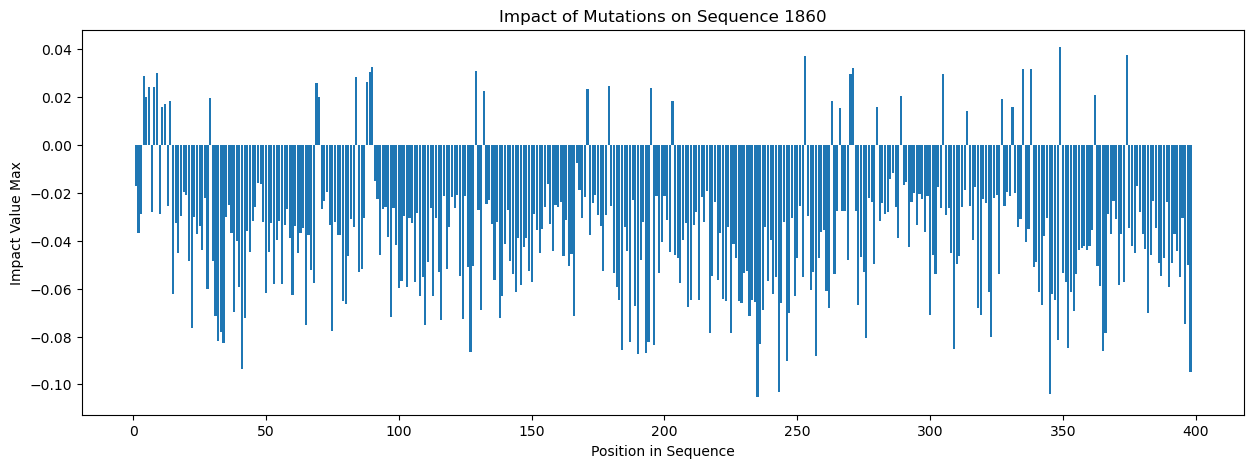
\includegraphics[width=1\linewidth]{5-small_mse_cold_hot.png}
    \caption{Single amino acid mutation effect on sequence 1860}
    \label{fig:seq1860}
  \end{figure}

\begin{figure}
    \centering
    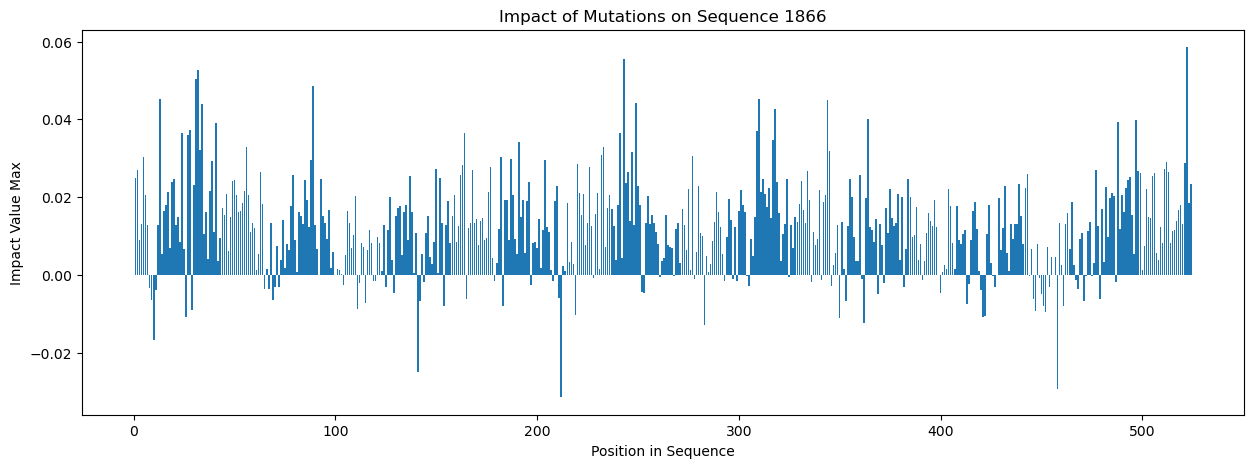
\includegraphics[width=1\linewidth]{5-high_mse_cold_hot.png}
    \caption{Single amino acid mutation effect on sequence 1041}
    \label{fig:seq1866}
  \end{figure}

Two main observations emerge from our experiment. First, the variation across all amino acid mutations is relatively consistent, with changes generally capped at a maximum of 0.10, which corresponds to a variation of up to 20\%. The second observation is that these variations can be both positive and negative, without a clear pattern emerging. These points are crucial as they offer insights into the model's operational dynamics.

Considering the role of specific amino acids in enzyme activity, it's known that only a limited number of amino acids within an enzyme are essential for facilitating a reaction, as explain in Section \ref{section:enzyme}. This implies that the presence or absence of these critical amino acids significantly influences the Michaelis constant, reflecting the enzyme's affinity for a substrate. Ideally, if an enzyme lacks these critical amino acids, the reaction would be severely impaired, leading to a substantially higher Michaelis constant. However, our data indicate that mutations result in values that remain close to the original predictions, suggesting that the model fails to capture the intricate interactions between the protein and the substrate accurately.
  
Enzymes are highly specific, and thus, it would be reasonable to expect that most mutated sequences would result in a higher Michaelis constant (indicating reduced affinity), with only a few exceptions potentially showing a lower constant (suggesting increased affinity). Such cases would be of great interest for enzyme engineering. Yet, the distribution of our results, featuring both positive and negative variations, does not align with this expectation, further highlighting the model's limitations in accurately modeling enzyme-substrate interactions.
  
To further investigate the model's performance, we next examine the distribution of substrates.

\subsection{Substrate Distribution Analysis}

Moving forward from the investigation into protein impacts, which revealed minimal influence on model predictions due to the model's inability to accurately predict the interaction between mutant proteins and substrates, our focus shifts towards the second input: the substrate. This section delves into what we call the substrate distribution, essentially examining the distribution of the Michaelis constant in relation to the different substrates.

Our initial step was to discern how the substrate distribution associated with high prediction errors contrasts with the overall distribution of substrates. Put simply, we aimed to understand how the Michaelis constant is distributed for substrates where the predicted values significantly deviate from their actual values, and to compare this with the broader dataset distribution.

\begin{figure}
    \centering
    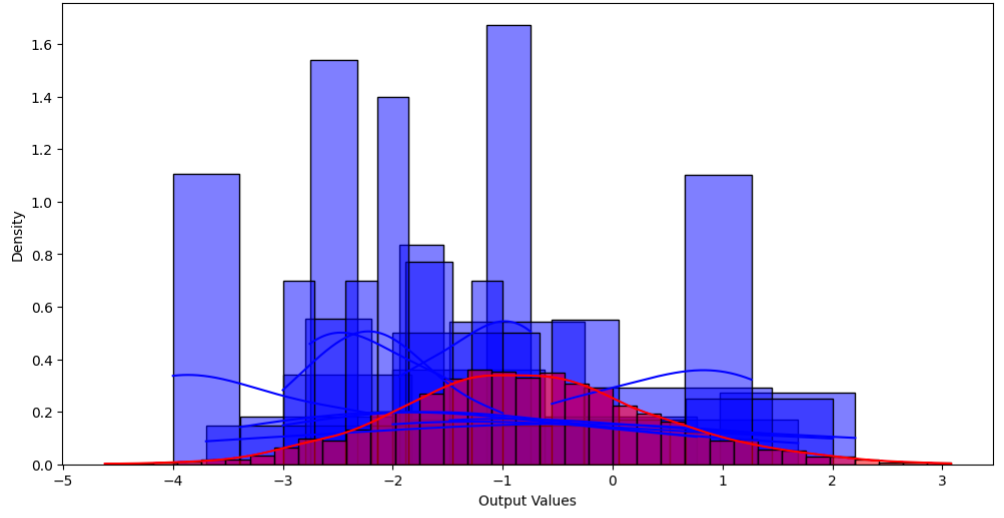
\includegraphics[width=\linewidth]{5-substrate-dist.png}
    \caption{Distribution of substrates with high prediction error}
    \label{fig:substratedist}
\end{figure}

In Figure \ref{fig:substratedist}, the distribution of the 10 substrates exhibiting the highest mean squared error (MSE) is depicted in blue, while the overall substrate distribution is shown in red. Despite the high error rates associated with these 10 substrates, their distribution aligns with the global substrate distribution. This observation suggests that the inaccuracies in predicting the Michaelis constant are not attributable to an atypical distribution of substrates, as the high errors do not correlate with distributions that deviate significantly from the global substrate distribution.

Further analysis of the ProSmith model's results reveals that the most substantial errors arise either from protein-substrate pairs not included in the training set (cold proteins and substrates) — as reflected by the high MSE for this subgroup — or from substrates and proteins that, despite being part of the training set, have Michaelis constants markedly divergent from the distribution specific to these substrates. This insight underscores the challenges the model faces in generalizing predictions across varying conditions, highlighting areas for potential improvement in its predictive accuracy and robustness.

\begin{figure}
    \centering
    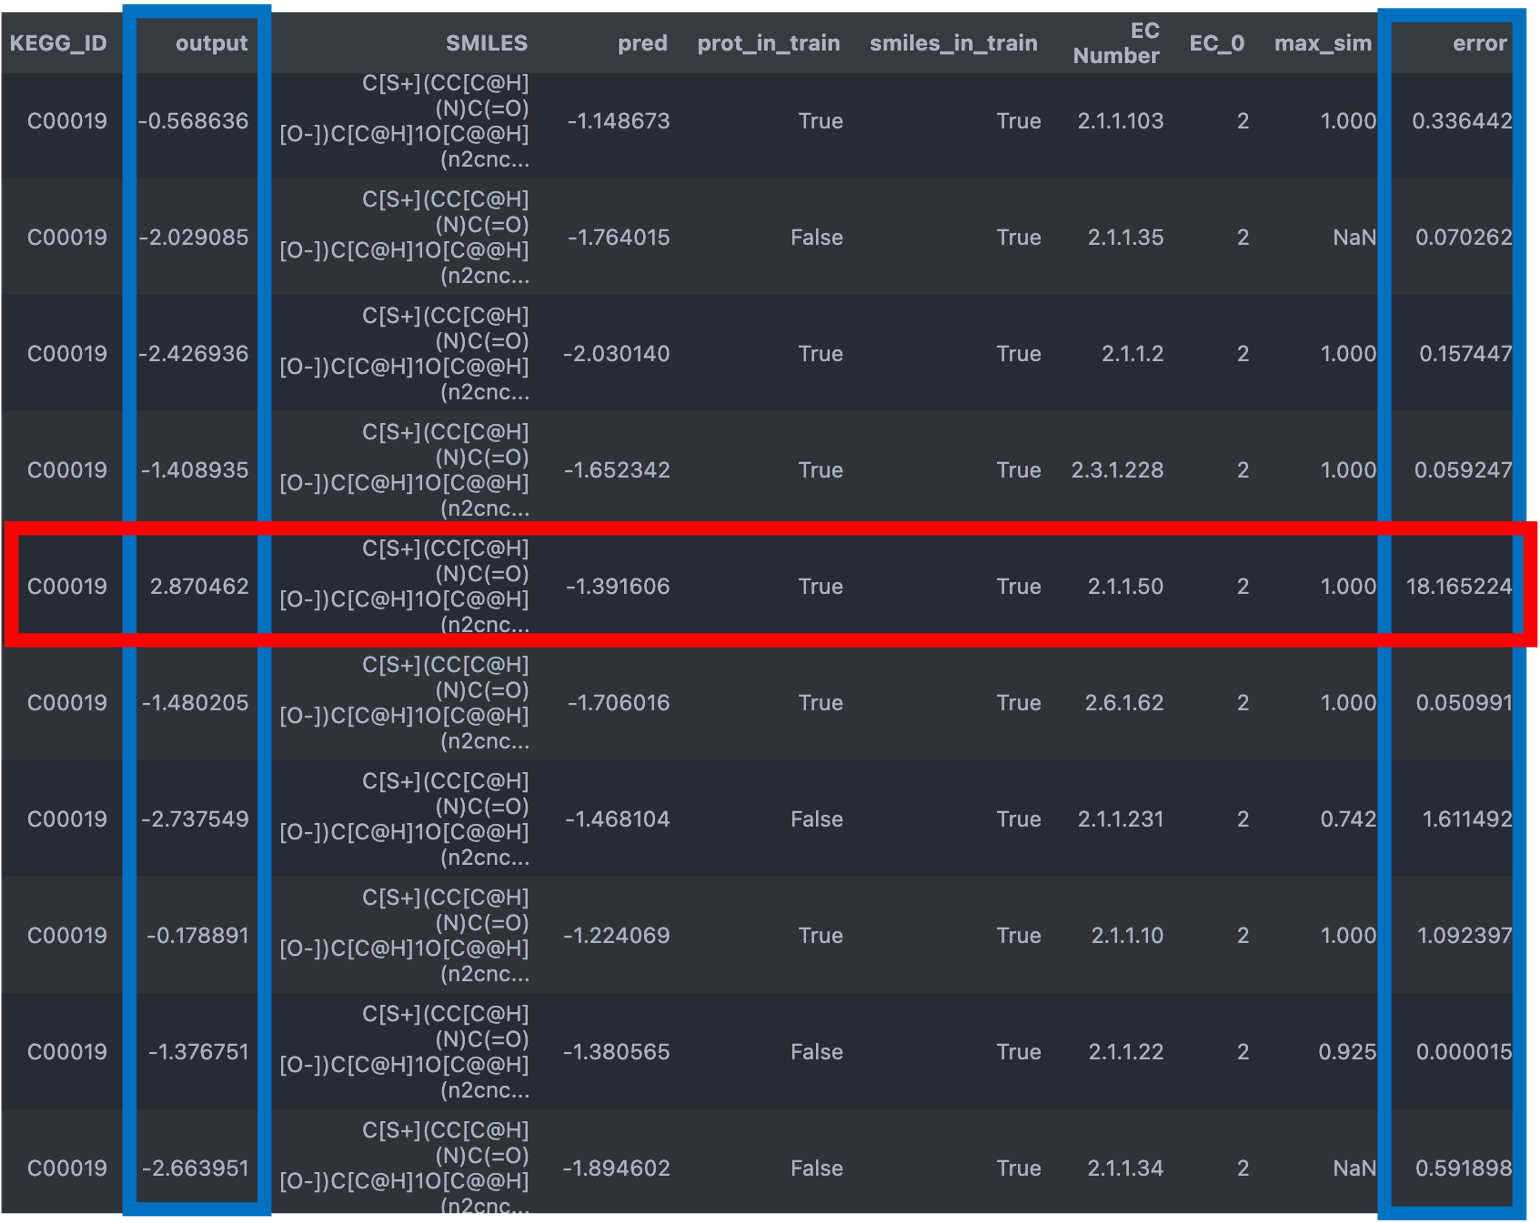
\includegraphics[width=1\linewidth]{5-results1.png}
    \caption{Results for the substrate S-Adenosylmethionine}
    \label{fig:sub1}
  \end{figure}

\begin{figure}
    \centering
    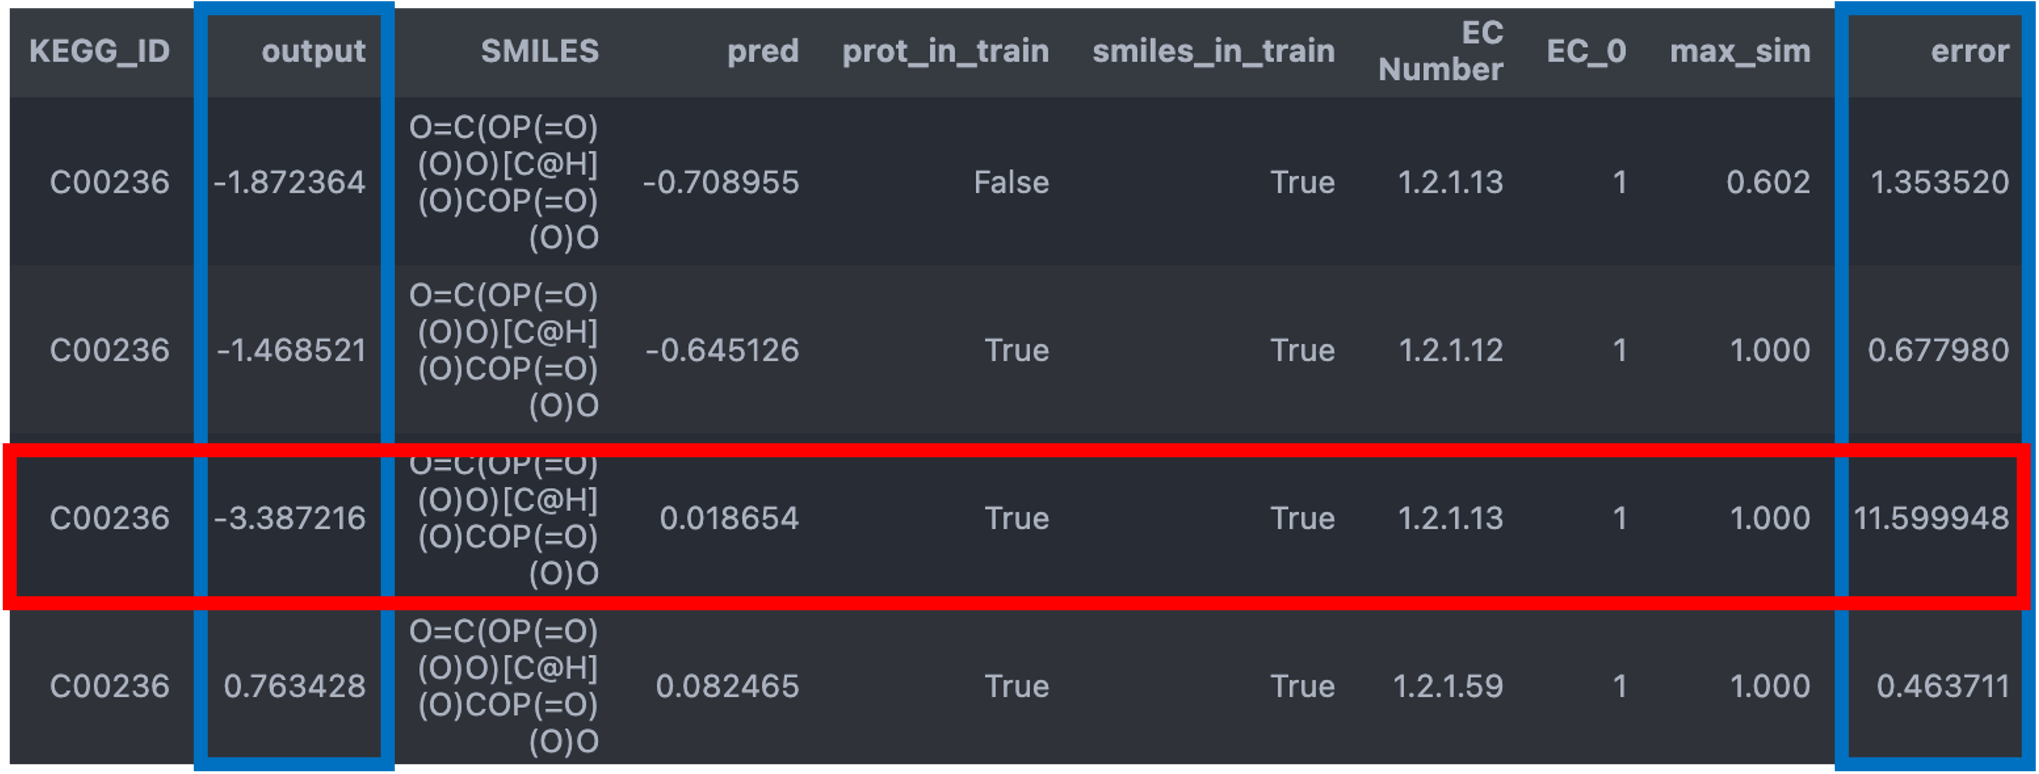
\includegraphics[width=1\linewidth]{5-results2.png}
    \caption{Results for the substrate Succinate semialdehyde}
    \label{fig:sub2}
  \end{figure}

Figures \ref{fig:sub1} and \ref{fig:sub2} examplify this discovery. As it is shown in red, we observe that for the same substrate, when the real Michaelis constant is outside of the general distribution of the substrate, the model is incapable of predicting this value properly and predicts instead a value inside the distribution of this substrate, showing the incapability of the model to predict properly the interaction between the enzyme and its substrate. However, this is a consequent problem as each substrate interact very differently between different enzymes and this element is essential to take into account, which is something ProSmith is incapable of doing.

\subsection{Analaysis Conclusions}

The detailed examination of single amino acid mutation effects reveals that the predicted Michaelis constant fluctuates within a narrow margin, disregarding the fundamental biological principle that an enzyme's specificity is compromised by mutations across its amino acid sequence. This observation signals ProSmith's inadequacy in capturing the essence of enzyme-substrate interactions.

Moreover, the analysis of substrate distribution further elucidates that the most pronounced prediction errors do not stem from substrates with atypical distributions. Instead, they arise from substrates with typical distributions that include some enzymes with markedly distinct Michaelis constants. This finding suggests that ProSmith's predictions are overly reliant on general substrate distribution patterns and lack the sophistication needed to model individual protein-substrate interactions accurately.

Despite ProSmith exhibiting superior performance metrics, such as MSE and coefficient of determination, the model demonstrates a clear deficiency in its ability to predict enzyme-substrate interactions precisely, indicating ample room for improvement. This limitation is particularly evident in its poor coefficient of determination of 0.082 for cold proteins and substrates, highlighting a significant challenge in generalization.

In subsequent chapters, our objective is to explore alternative methods to address these issues. Our aim is to enhance the model's capacity for accurate prediction and generalization across diverse enzyme-substrate interactions, thereby overcoming the limitations observed in ProSmith's current implementation.

% !TeX root = ../thuthesis-example.tex

\chapter{Sequence-based Method}

\section{Introduction}

As of today, only sequence-based model exists for the prediction of the Michaelis constant. Some (Km pred1) use
simple embeddings to represent the protein sequences. Other such as (ENKIE) use Bayesian Multilevel Models (BMMs)
to capture a simple hierarchy of enzyme properties. Finally, the state-of-the-art model ProSmith pre-trains a
large enzyme-specific protein models and uses embeddings from existing large protein models. 

In this chapter, we present SeqKm a deep learning model that makes use of existing large protein models without
pretraining. This not only allows for fast training and prediction as there is no need for pretraining but also
offer better performances by leveraging the protein knowledge retained by large protein models.

To demonstrate our method applicability to Michaelis constant prediction, we analyze the sequence-based
model performance compared to the state-of-the-art models in this field. Even though this model
does not outperform ProSmith, it shows equal performances on the new curated test set, indicating our
model's better ability to generalize and showing promissing results for the ensemble method.

\section{Methods}

We now describe our input representation, model achitecture, training details, and results. 
Figure \ref{fig:seqkm} provides an overview of our method.

\begin{figure}
  \centering
  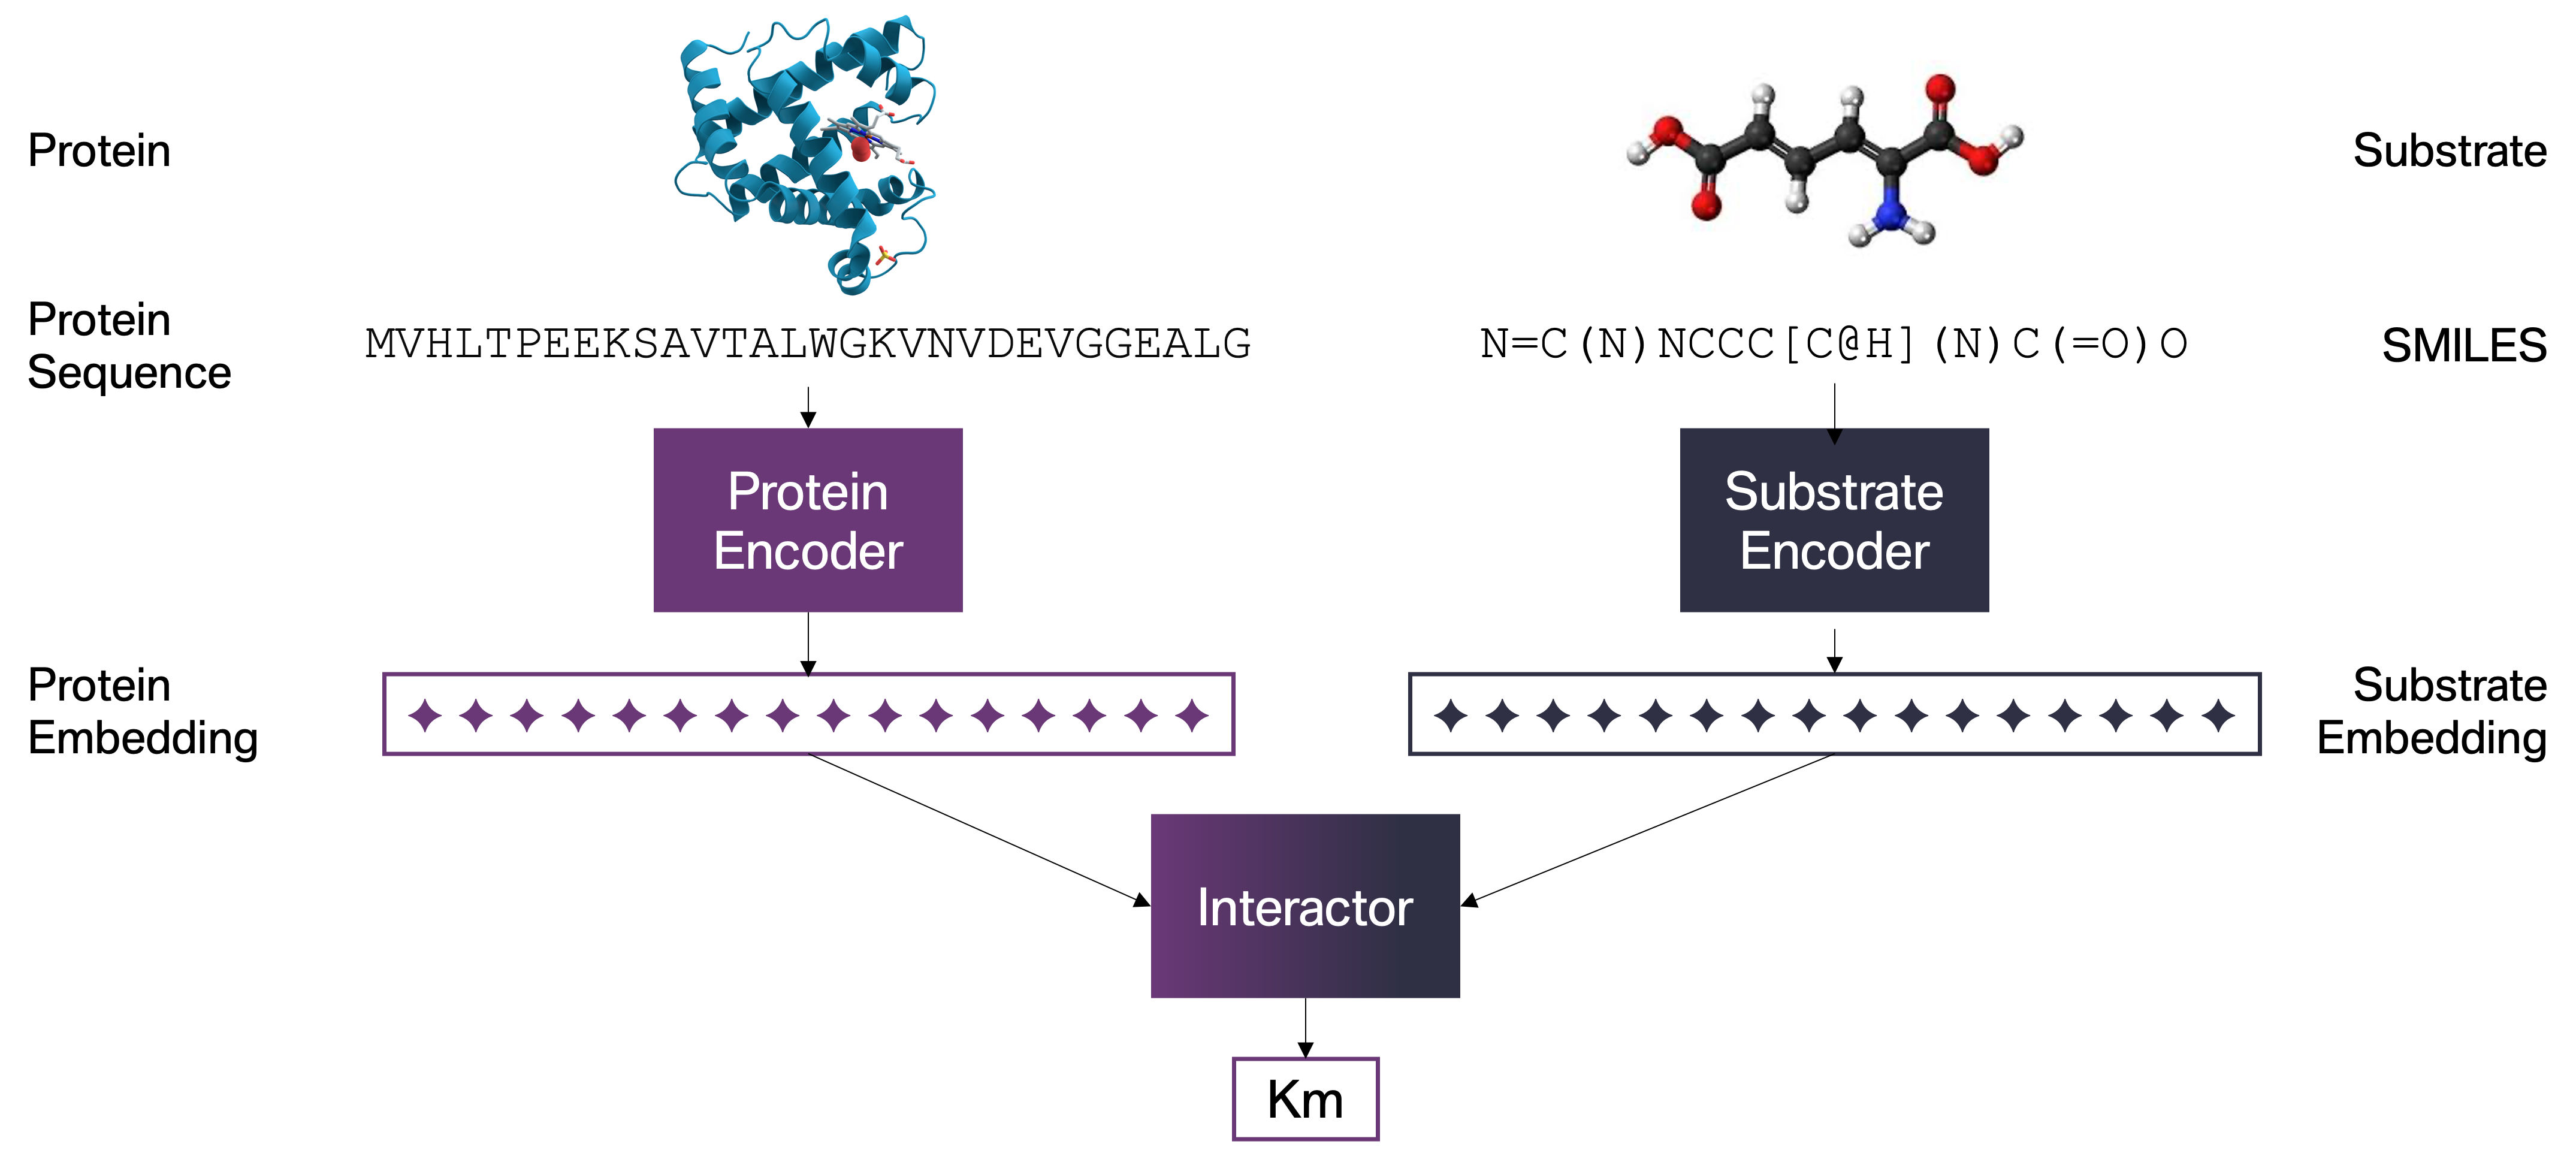
\includegraphics[width=1\linewidth]{2-sequence_architecture.png}
  \caption{Overview of SeqKm}
  \label{fig:seqkm}
\end{figure}

\subsection{Input representation}

We are given a protein sequence of length $n$ $P=a_1a_2a_3...a_n$ where $a_i$ represents the amino acid
at position $i\in\{1,..,n\}$ and each $a_i$ is an element from the set of 20 standards amino acids to
which we added an unknown amino acid $X$: $A=\{A,C,D,E,F,G,H,I,K,L,M,N,P,Q,R,S,T,V,W,Y,X\}$.

As a string cannot directly be processed by a deep learning model, a tokenization step is necessary. As
the ProtT5-XL model will be used, its tokenizer will also be used to prepare the protein sequences \cite{prottrans}.
The ProtT5-XL tokenizer is made on a vocabulary containing all the 20 amino acids but also other unsure or less
common amino acids such as B that refers to asparagine (N) and aspartic acid (D) when the specific
amino acid cannot be determined. It also has a padding token <pad>, an unknown token <unk>, a end
token </s> to indicate the end of the sequence, and some additional tokens for special cases.

Hence, all protein sequences are first truncated or padded to length 1023 and then tokenized to have inputs of
length 1024: 1023 amino acids or pad tokens <pad> and the end token </s>. This input can be used for downstream
applications.

We are also given a substrate string in its SMILES form. This can be defined as a $S=c_1c_2c_3...c_n$
where $c_i$ represents the chemical symbol for the atom at position $i\in\{1,...,n\}$ in the SMILES
sequence, or a symbol representing a bond or branching in the molecule.

Similarly, it first needs to be processed in a format that can be processed by a statistical model. To do so,
we use the Morgan Fingerprints that represent a small molecule in a way that can easily be used for computational
tasks such as ours. We selected a vector size of 1024 to be consistent with the size of the protein sequence. We
also choose to use a radius size of 1, indicating that each atom of the molecule is updated only once based on its
immediate neighbors.

We know have two inputs that can be processed by a machine learning model.

\subsection{Model Architecture}

Our model is composed of three modules: a protein encoder that encode the protein, a substrate encoder that
encode the substrate, and an interactor that makes the encoded protein and the encoded substrate interact.

The protein encoder is composed of the ProtT5-XL model to which we relaxed the 2 last layers during the training.
Relaxing is a selective fine-tuning strategy that allows to slightly adjust certains weights of a pretrained model 
to better perfom on our specific task. The decision of relaxing only the 2 last layers of the model is based on
the assumption that these layers contain the most task-specific information, while ealiest layers usually capture
universal features. This not only render the training faster are only a few weights need to be updated during the
fine-tuning process while still making the model adapted to our specific task.

The protein encoder output a matrix of size $1024\times 1024$ with the first one being the length of the sequence,
padded or not, and the second being the embedding dimension which is 1024. Technically, this mean that every
amino acid has an embedding of size 1024. Considering we are only looking for an embedding per protein sequence
and not per amino acid, we use the common technique of averaging on the amino acid dimension, leaving us with a
single vector of length 1024.

The substrate encoder for this model is simply a dummy model that does not modify the input as it was already
processed as a Morgan Fingerprints, which is already a reprensetation of the substrate as a vector of length 1024.

Finally, the interactor is a multilayer perceptron of 2 dense layers of size 256 and 128. It takes as input the
concatenated protein embedding and substrate embedding and pass it through these 2 layers to finally output a single
value, the Michaelis constant $K_m$.

\section{Training details}

We trained and validated our model using the dataset described in Section \ref{sec:dataset} as well as the new
test dataset that we currated and that contains data from 2022 to 2024. The training set contains roughly 8k
protein-substrate pairs and their $K_m$ value. The validation and testing set contains about 1k and 2k pairs
respectively. 

We trained our model over 300 epochs using the Adam optimizer with $\beta_1=0.9$ and $\beta_2=0.999$, and an initial
learning rate of $5\times10^{-4}$. The learning rate follows a cosine schedule, including a warmup phase of 200
steps to gradually increaser the learning rate from zero to the initial set value, ehnancing the model's convergence
stability. Training and validation batch sizes are set to 256 and 32 per device, respectively, to efficiently
utilize computational resources while maintaining an appropriate balance between speed and memory usage. 

Additionally, we leverage a cosine learning rate scheduler to adjust the learning rate dynamically, 
encouraging better fine-tuning and generalization as training progresses. To monitor the model's performance 
and ensure robustness, we log metrics every 20 steps and save the model's state every 500 steps. 
Evaluation is conducted at each step, allowing for continuous monitoring of the model's effectiveness on 
validation data. 

Finally, after looking at the best metrics for the validation test, we reverted to the saved model of the
 17th epoch. 

 \section{Results}

 Using the model and the training strategy presented above, we obtain a MSE of 0.700 and a $r^2$ of 0.493 
 as well as the following hot/cold results for the test set:

 \begin{table}[ht]
  \centering
  \begin{tabular}{lcccccc}
  \hline
   & \multicolumn{3}{c}{\textbf{Hot substrate}} & \multicolumn{3}{c}{\textbf{Cold substrate}} \\
   & Samples & MSE & R\(^2\) & Samples & MSE & R\(^2\) \\ \hline
  \textbf{Hot protein}  & 1192 & 0.642 & 0.485 & 64 & 0.821 & 0.449 \\
  \textbf{Cold protein} & 985 & 0.708 & 0.536 & 98 & 1.250 & -0.004 \\ \hline
  \end{tabular}
  \caption{SeqKm results on the test set}
  \label{tab:summary_performance}
 \end{table}



For the new test set, we obtain:

\begin{table}[ht]
  \centering
  \begin{tabular}{lcccccc}
  \hline
   & \multicolumn{3}{c}{\textbf{Hot substrate}} & \multicolumn{3}{c}{\textbf{Cold substrate}} \\
   & Samples & MSE & R\(^2\) & Samples & MSE & R\(^2\) \\ \hline
  \textbf{Hot protein} & 40 & 0.787 & 0.472 & 30 & 0.851 & -0.255 \\
  \textbf{Cold protein} & 1117 & 0.884 & 0.478 & 102 & 2.066 & -0.006 \\ \hline
  \end{tabular}
  \caption{SeqKm results on the new test set}
  \label{tab:updated_summary_performance}
\end{table}

Our method offer better performances only for 1 out of the 4 models of our benchmark, which indicates 
possible improvements.
% !TeX root = ../thuthesis-example.tex

\chapter{Structure-based Method}

\section{Introduction}

So far in the literature, no model have been using protein structural information for predicting the Michaelis
constant. However, it is known that the protein structure, also known as the terciary structure of a protein - in
opposition to the protein sequence which is known to be the primary structure of a protein - is essential. Indeed,
even though the sequence contains all the necessary information for a protein expression, many models cannot
extract all the necessary meaningful information from the primary structure and require more information. This is
where the protein structure can improve the predictions. 

Many research efforts have been put into predicting the structure of proteins such as AlphaFold or ESMFold and
these structure can be use down the line for concrete applications such as the acceleration of design 
of a drug to treat hepatocellular carcinoma (HCC), the most common type of primary liver cancer (https://www.artsci.utoronto.ca/news/new-study-uses-alphafold-and-ai-accelerate-design-novel-drug-liver-cancer)
Since the release of the AlphaFold database that contains over 200 millions structures, these methods have multiplied.
However, so far they haven't been used for predicting the Michaelis constant and our work is, to our knowledge, 
the first one to explore the use of protein structure for $K_m$ prediction.

In this chapter, we present StuctKm, a deep learning model that makes use of the protein structures of the
AlphaFold database. This method does not require any pretraining, making it fast and easily trainable. 

While the global results only outperform one out of our four benchmark models, it shows better performance 
than the current best model on the most important subset: cold proteins and cold substrates.

\section{Methods}

We now describe our data preprocessing step, input representation, model achitecture, training details, and results. 
Figure \ref{fig:seqkm} provides an overview of our method.

\begin{figure}
  \centering
  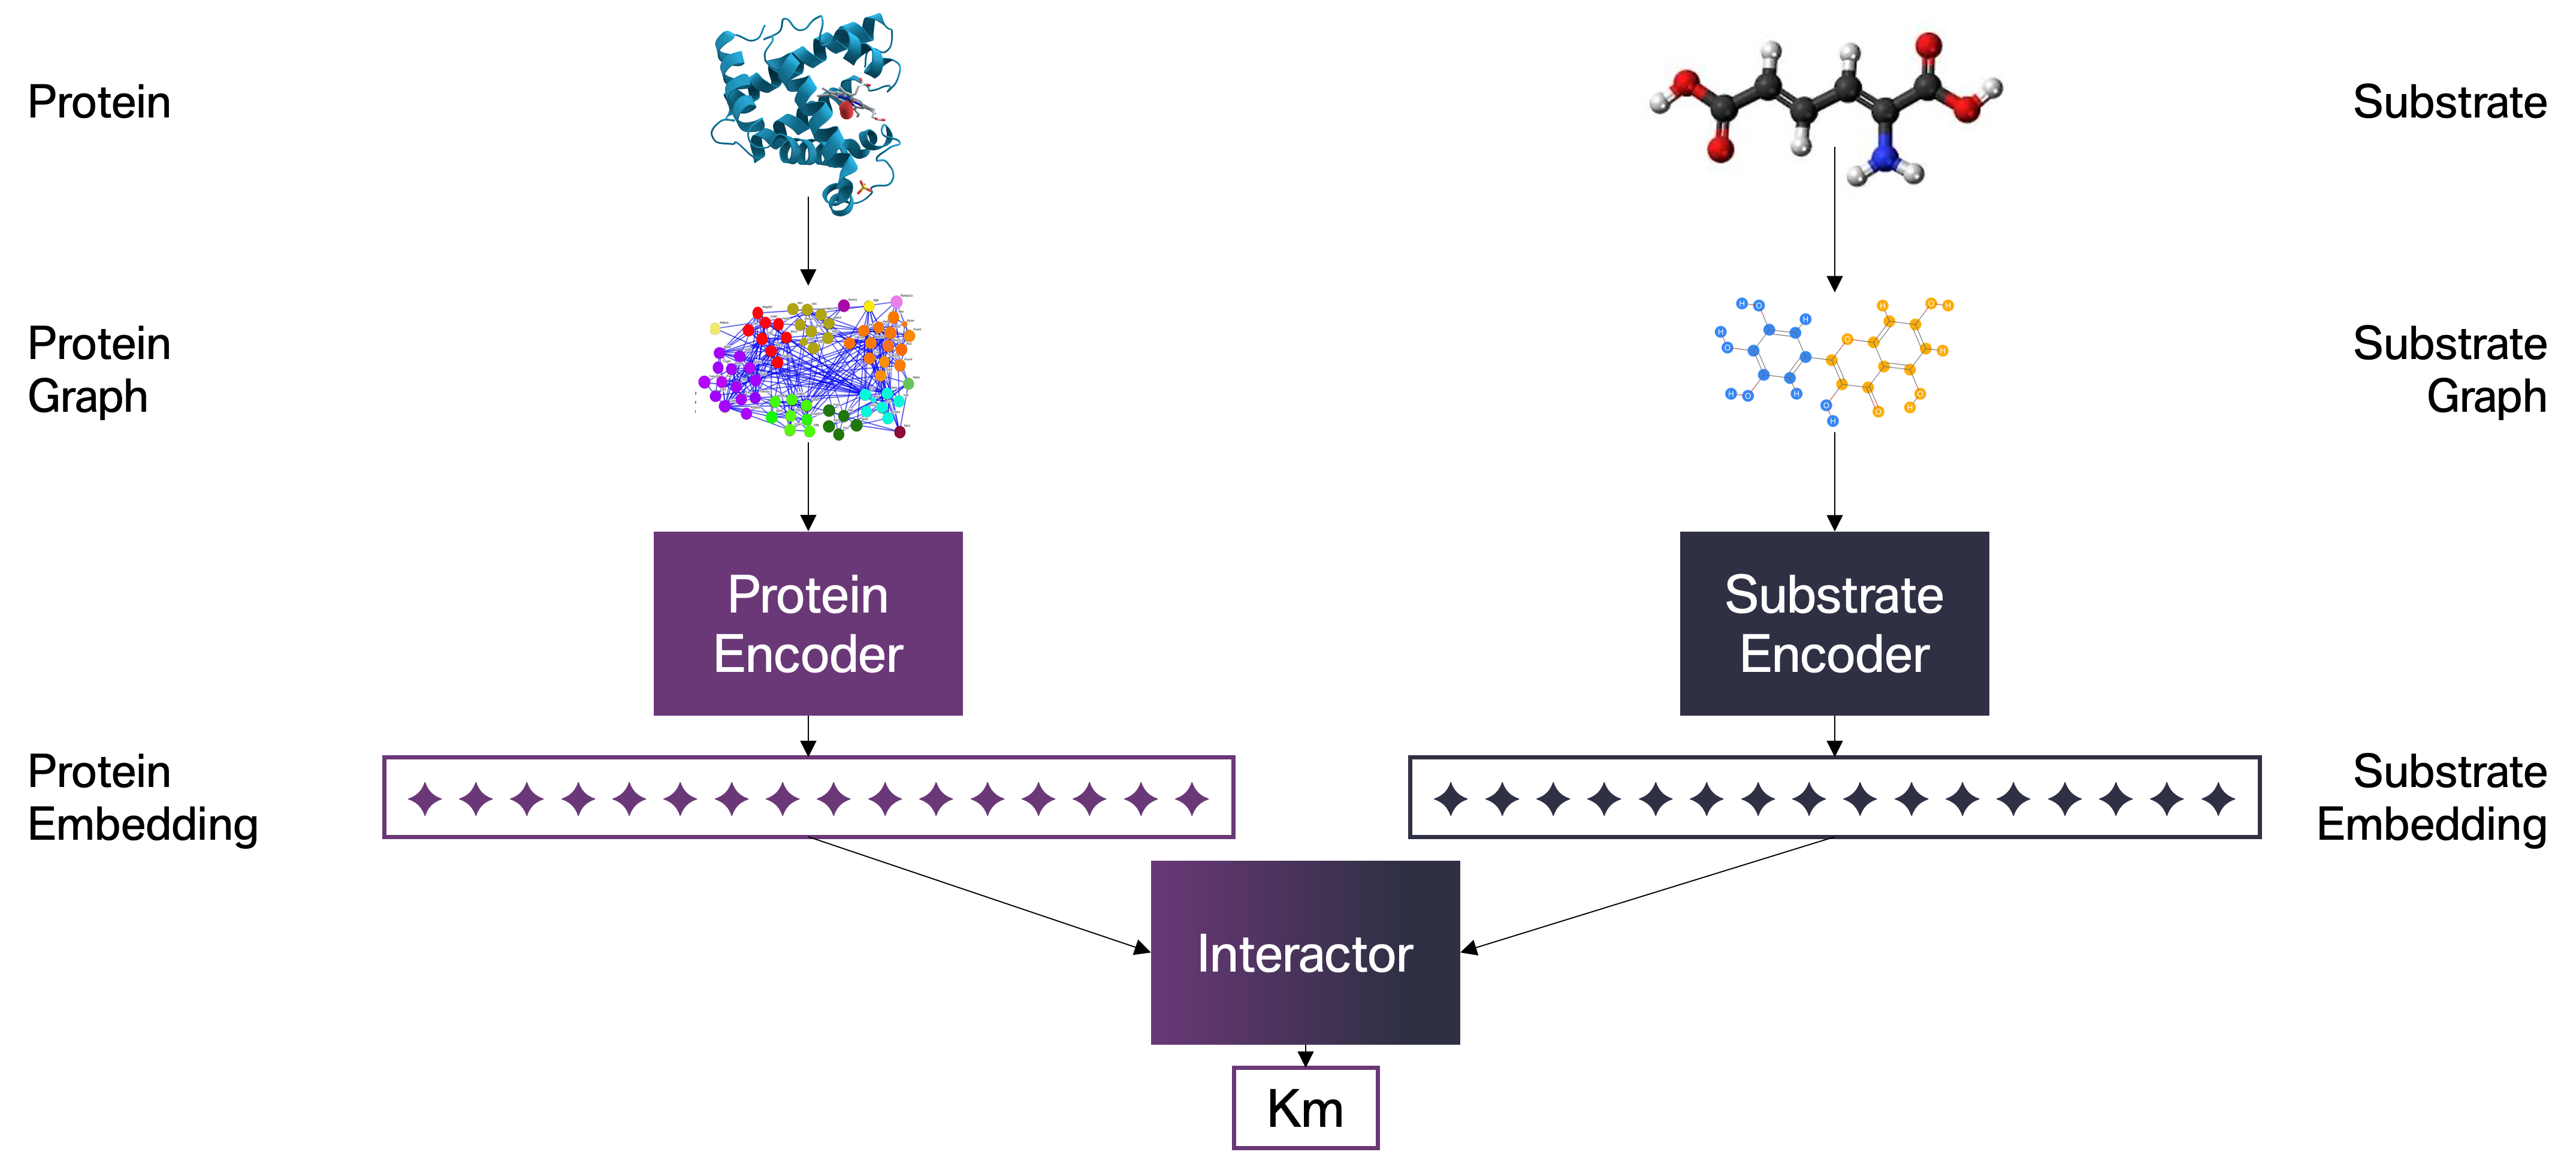
\includegraphics[width=1\linewidth]{3-structure_architecture.png}
  \caption{Overview of StructKm}
  \label{fig:structkm}
\end{figure}

\subsection{Data Preprocessing}

While the sequences were already present in the $K_m$ dataset, the structures were not. It was therefore necessary
for us to retrive them in order to use them for our structure-based model. To do so, we followed these steps:
\begin{enumerate}
  \item Identify the UniProtID of each sequence of our dataset. If it doesn't exist, find the UniProtID with the 
  highest sequence similarity rate.
  \item Download the PDB file from the AlphaFold database.
\end{enumerate}

\subsubsection{Retriving UniProtIDs}
First, we need to retrive the UniProtIDs of all the sequences of our dataset. The reason behind this is that
AlphaFold contains almost all the structure of the UniProt database, making it easy to obtain the structure.
Indeed, using only the sequence as a tool to find the relevant structure in the AlphaFold database led to finding
less than 50\% of the structures for our sequences.

The Universal Protein Resource (UniProt) is a comprehensive resource for protein sequence and annotation. The 
UniProt database is composed of the UniProt Knowledgebase (UniProtKB), the UniProt Reference Clusters (UniRef), 
and the UniProt Archive (UniParc). Specifically, UniProtKB is a comprehensive resource for protein sequence 
and annotation data. It consists of two sections: UniProtKB/Swiss-Prot and UniProtKB/TrEMBL. 
UniProtKB/Swiss-Prot provides manually annotated records with information verified by experts, 
focusing on accuracy and reliability. These annotations include function descriptions, 
domain structure, post-translational modifications, variants, and many other biological insights. 
UniProtKB/TrEMBL, on the other hand, contains automatically annotated records that have not yet been 
reviewed by humans. In this work, we will only use UniProtKB/Swiss-Prot.

To identify the UniProtID related to our protein sequences, we used a bioinformatics program called 
Basic Local Alignment Search Tool (BLAST). It can be used for comparing protein or nucleotides to sequence databases.
Specifically, we used blastp that is designed for proteins only and we compared our sequences to the 
UniProtKB/Swiss-Prot database. 

For 80\% of our sequences, we found an above 100\% sequence similarity, indicating a perfect match between our
sequence and the sequence in the UniProtKB/Swiss-Prot dataset. For the 20\% remaining, the sequence similarity is
still relatively high (above 90\% for a large proportion), indicating a high similarity. Even though the match is
not perfect, we will use these UniProtIDs and related structures and will detail in the discussion section their
impact on the results.

\subsubsection{Downloading the PDB files}

Second, once all the UniprotIDs of our sequences have been retrieved, we can download their PDB files.

A Protein Data Bank (PDB) file is a text file that contains the three-dimensional structures of molecules like
proteins and nuclic acids. These files include atomic coordinates, secondary structure assignments, 
and atomic connectivity, among other experimental metadata. The PDB format is a legacy file format that 
has been succeeded by the mmCIF format, but it is still widely used and supported by many molecular 
visualization software applications and will be used in this work.

The AlphaFold database offers all the structures predicted by the AlphaFold 2 model in PDB and mmCIF formats. 
We therefore downloaded all the structures of our UniProtIDs. 

\textbf{Note:} While UniprotIDs are unique, they might refer to the same sequences. This means that one sequence can have
several UniProtIDs. However, in the AlphaFold database, for most of the data, the structure was only generated 
for one of these UniProtIDs. Hence, before downloading the structure, we added a step to make sure to have 
the UniprotID related to the structure in the AlphaFold database.

\subsection{Input representation}

Let a protein structure be defined as a tuple $P = (S, \Sigma, \Theta, \Phi)$ where:


\begin{itemize}
  \item $P=a_1a_2a_3...a_n$ is the primary structure, a sequence of amino acids where each 
  $a_i \in A$ for $i \in \{1,..,n\}$, and $A=\{A,C,D,E,F,G,H,I,K,L,M,N,P,Q,R,S,T,V,W,Y,X\}$ is the set of 
  standard amino acids including an unknown amino acid $X$.
  \item $\Sigma = {\sigma_1, \sigma_2, ..., \sigma_m}$ represents the secondary structure, a set of 
  local structures commonly found in proteins, such as alpha helices ($\alpha$-helices) and 
  beta strands ($\beta$-strands), where each $\sigma_j$ is a tuple $(type, start, end)$ 
  with $type \in {\alpha, \beta}$ indicating the type of secondary structure, and $start, end \in \{1,..,n\}$ 
  defining the positions in the primary sequence $P$ where the structure begins and ends.
  \item $\Theta = {\theta_1, \theta_2, ..., \theta_n}$ where each $\theta_i$ corresponds to an amino acid 
  in the protein and is defined as a tuple $\theta_i = (a_i, A_i)$. $a_i \in A$ denotes the type of amino acid for 
  the $i^{th}$ position in the protein sequence. $A_i = {(\alpha_{ij}, x_{ij}, y_{ij}, z_{ij})}_{j=1}^{M_i}$ 
  represents the set of atoms for the $i^{th}$ amino acid, where $\alpha{ij}$ is the atom type 
  (e.g., carbon, nitrogen, oxygen), and $(x_{ij}, y_{ij}, z_{ij})$ are the spatial coordinates of 
  the $\alpha_{ij}$ atom in three-dimensional space. $M_i$ is the total number of atoms 
  in the $i^{th}$ amino acid.
  \item $\Phi = \{S_1, S_2, ..., S_k\}$ represents the quaternary structure, a set of protein subunits where 
  each $S_i$ is a tertiary structure, indicating how multiple polypeptide chains (subunits) 
  assemble into a functional protein complex.
\end{itemize}

Our goal is to make use of the protein as a PDB file and no longer rely on only its primary structure but 
also its terciary structure. To do so, we will use a graph representation of a protein. Each amino acid will
be represented as a node and the edges between the nodes will depends on the distance to the nodes. If the
alpha-carbons of two amino acids are less than 6 {\AA} away, then there will be an edge between them. 
If they are apart of more than 6 {\AA}, then they will not be connected. Later on, we will use Graph Neural Networks
and the message-passing paradigm that allows use to connect and allow interactions between amino acids that
might be far from each other in the protein sequence but close in its three-dimensional structure, hence making 
use of the structural information.

Furthermore, we will use the ESM2 model to generate the embeddings of the nodes of our protein graph. As the nodes
of our protein graph represent amino acids, we can use ESM2 to generate the embedding vector for each amino acid
of the sequence, that we then feed to the relevant node. This allows to add sequential information to our graph.

At the end, we obtain a protein graph with amino acids as nodes and the ESM2 embedding and the edges depending on
the structural proximity of the amino acids. We can then feed these graphs to a GNN.

For the substrate, we will once again use the Morgan Fingerprints as they represent the substrates in a way 
that can easily be used for computational tasks.

We know have two inputs that can be processed by a machine learning model.

\subsection{Model Architecture}

Similarly to our sequence-based model, our structure-based model is composed of three modules: a protein encoder 
that encode the protein, a substrate encoder that encode the substrate, and an interactor that makes the 
encoded protein and the encoded substrate interact. The main difference lies in the protein encoder.

The protein encoder is a Graph Neural Network and specifically a Graph Convolutional Neural Network (GCN). We also 
tried a Graph Attention Neural Network (GAN) and obtain similar results so we will focus here on the GCN. Our GCN
has 2 graph convolution layers that allow message passing between the nodes by aggregating neighborhood 
information. The first convolution layer is followed by a ReLU activation and a dropout layer to enhance 
feature representations while preventing overfitting. A subsequent graph convolution layer further refines 
these features, which are then globally aggregated to yield a singular, graph-level output. This output of size 128
encapsulates the structural and feature-based information of the entire graph and is one of the two inputs of 
our interactor. 

The substrate encoder is similar to the sequence-based model, the only difference being that the Morgan Fingerprints
is now a vector of size 128 and not 1024, to be consistent with the size of the protein embedding.

Finally, the interactor is a multilayer perceptron of 2 dense layers of size 256 and 128. It takes as input the
concatenated protein embedding and substrate embedding and pass it through these 2 layers to finally output a single
value, the Michaelis constant $K_m$.

\subsection{Training details}

We trained and validated our results on the same dataset we used for the sequence-based model. The only difference
being that the sequences are replaced by protein graphs. The prediction to make however is exactly the same and 
therefore the exact same methodology can be used for evaluation.

Once again, we trained our model over 300 epochs using the Adam optimizer with $\beta_1=0.9$ and $\beta_2=0.999$, and an initial
learning rate of $5\times10^{-4}$. The learning rate follows a cosine schedule, including a warmup phase of 200
steps to gradually increaser the learning rate from zero to the initial set value, ehnancing the model's convergence
stability. Training and validation batch sizes are set to 256 and 32 per device, respectively, to efficiently
utilize computational resources while maintaining an appropriate balance between speed and memory usage. 

Additionally, we leverage a cosine learning rate scheduler to adjust the learning rate dynamically, 
encouraging better fine-tuning and generalization as training progresses. To monitor the model's performance 
and ensure robustness, we log metrics every 20 steps and save the model's state every 500 steps. 
Evaluation is conducted at each step, allowing for continuous monitoring of the model's effectiveness on 
validation data. 

Finally, after looking at the best metrics for the validation test, we reverted to the saved model of the
 22nd epoch. 

 \section{Results}

 Using the model and the training strategy presented above, we obtain a MSE of 0.712 and a $r^2$ of 0.485 
 as well as the following hot/cold results for the test set:

 \begin{table}[ht]
  \centering
  \begin{tabular}{lcccccc}
  \hline
   & \multicolumn{3}{c}{\textbf{Hot}} & \multicolumn{3}{c}{\textbf{Cold}} \\
   & Samples & MSE & R\(^2\) & Samples & MSE & R\(^2\) \\ \hline
  \textbf{Hot seq}  & 1135 & 0.644 & 0.485 & 64 & 0.795 & 0.475 \\
  \textbf{Cold seq} & 1042 & 0.746 & 0.505 & 98 & 1.066 & 0.135 \\ \hline
  \end{tabular}
  \caption{StructKm results on the test set}
  \label{tab:summary_performance}
\end{table}

For the new test set, we obtain a total MSE of 1.257 and a total $r^2$ of 0.286. In details:

\begin{table}[ht]
  \centering
  \begin{tabular}{lcccccc}
  \hline
   & \multicolumn{3}{c}{\textbf{Hot}} & \multicolumn{3}{c}{\textbf{Cold}} \\
   & Samples & MSE & R\(^2\) & Samples & MSE & R\(^2\) \\ \hline
  \textbf{Hot seq}  & 40 & 1.439 & 0.067 & 30 & 0.827 & -0.190 \\
  \textbf{Cold seq} & 1117 & 1.175 & 0.306 & 102 & 2.202 & -0.078 \\ \hline
  \end{tabular}
  \caption{StructKm results on the new test set}
  \label{tab:summary_performance}
\end{table}

The lower results for the new test set are due to a low similarity (34\%) similarity for the UniProtID 
matches with the sequence using BLAST for this set. Hence, the structures do not accurately represent the
proteins, introducing noise into the data and lowering the performances.

Overall, our method offer better performances only for 1 out of the 4 models of our benchmark, which indicates 
possible improvements. However, we also notice the 0.135 for the cold proteins and cold substrates, which is
one of the most important of our work as our goal is to find new possible drugs and hence it must be a cold protein
and a cold substrate. This value is above the 0.11 of ProSmith and is extremely important for our work. We will
discuss it in more details in the discussion part.

\section{Pocket Detection Model}

In this section, we present an alternative to the structure-based model. So far, we have always presented
a model using the entire protein. However, as we explained it in Section \textcolor{red}{literature review},
the reaction between the enzyme and the substrate operate in a specific part of the protein which is called
a pocket. Hence, we believe that if we can efficiently find the pocket for each protein and use it instead of
the entire sequence, we may obtain better results and reduce the noise inputed by parts of the protein that 
are not relevant for predicting the Michaelis constant. 

To do, different methods can be used and we will focus on fpocket. fpocket is an open-source command line
tool designed for the identification and analysis of protein pockets. It is widely used in computational
biology as it predicts potential binding sites on the surface of protein structures and do so very quickly
compared to other more novel and more computaionally expensive deep learning methods for pocket detection.

We therefore used fpocket to identify the best pockets for each of our protein structure, selected the top
one pocket, and then took the subgraph
corresponding to this predicted pocket and used it as an input in our structure-based model. The subgraph 
being a graph, the model didn't required any modification. With a similar methodoly than previously, we
trained our model and obtained an MSE of 0.770 and a correlation coefficient of 0.443. Specifically,
we have:

\begin{table}[ht]
  \centering
  \begin{tabular}{lcccccc}
  \hline
   & \multicolumn{3}{c}{\textbf{Hot}} & \multicolumn{3}{c}{\textbf{Cold}} \\
   & Samples & MSE & R\(^2\) & Samples & MSE & R\(^2\) \\ \hline
  \textbf{Hot seq}  & 1192 & 0.672 & 0.461 & 64 & 0.934 & 0.373 \\
  \textbf{Cold seq} & 985 & 0.823 & 0.461 & 98 & 1.324 & -0.063 \\ \hline
  \end{tabular}
  \caption{SeqKm results on the test set}
  \label{tab:results_pocket_test}
 \end{table}

For the new test set, we have an MSE of 1.233 and a correlation coefficient of 0.300. Specifically,

\begin{table}[ht]
  \centering
  \begin{tabular}{lcccccc}
  \hline
   & \multicolumn{3}{c}{\textbf{Hot}} & \multicolumn{3}{c}{\textbf{Cold}} \\
   & Samples & MSE & R\(^2\) & Samples & MSE & R\(^2\) \\ \hline
  \textbf{Hot seq}  & 40 & 1.322 & 0.114 & 30 & 0.873 & -0.289 \\
  \textbf{Cold seq}& 1117 & 1.166 & 0.312 & 102 & 2.033 & 0.010 \\ \hline
  \end{tabular}
  \caption{SeqKm results on the test set}
  \label{tab:results_pocket_new_test}
 \end{table}

As we observed, our results for the pocket model are lower than for the full protein. To understand why in
details, we made an analysis on the pockets we found, the main goal being to determine if the pockets we found
were actual pockets. This task is difficult as our protein structure are generated by AlphaFold and hence do
not contain any annotations about the real pocket where the enzymatic reaction happens. However, some of the
proteins possess experimentally determined crystallographic structures where the pocket is anotated. From 
these, we can have a better understanding of our model and its capabilities.

Hence for all the protein which had a known crystallographic structure, we retrieved them from the Protein 
Data Bank and run the fpocket algorithm on top of it to verify if the real pocket where indeed at the 
locations predicted by the algorithm. We manage to retrieve around 2,000 real structures which is about 
20\% of our dataset. While it is only a subset of our dataset, we should still be able to obtain meaningful
insights that may explain the lower performance.

Running the fpocket algorithm on these crystallographic structures, we obtain the following results:
\begin{itemize}
  \item Top 1: 55.17\%
  \item Top 3: 69.62\%
  \item Top 5: 72.96\%
\end{itemize}
This means that half of the time, the pocket we detect with fpocket and that we use in our downstream application
is not the real pocket. Hence our training data includes some incorrect data which seems to explain why
our model is performing more poorly using pockets that the entire structure.

While the idea of using the local information (pocket) instead of the global information (full structure)
seems very interesting and makes biological sense, it does not seems to be possible using only the best pocket
predicted by fpocket. 
Using the top 3 or top 5 pockets may be useful but would need a tailored approach to feed these pockets to
the model.
It could also be possible to use different models for pockets detection but we decided to not continue in this 
direction as we believe that decent results can be obtained by using the global information only, as described
in the following chapter.
% !TeX root = ../thuthesis-example.tex

\chapter{Ensemble method}

\section{Introduction}

As mentioned in the introduction of the previous chapter (Chapter \ref{chap:4}), no method using structural information exists for the prediction of the Michaelis constant. Hence, methods combining both sequential and structural information also do not exists. However, in the field of protein design, a few models started using both sequential and structural features and have shown promising results such as the work of \citeauthor{wu2023a} that use structure-sequence co-design for antibodies and offer state-of-the-art results in the field.

In this chapter, we present the first ensemble method that uses both sequential and structural information for Michaelis constant prediction, SeqStructKm. Not only does it outperforms 3 out of the 4 current-state-of-the art models but it also outperforms the best model, ProSmith, on the cold proteins and cold substrates subset, which is of significant importance for drug design. This demonstrates the efficacy of our method and promising opportunities for future work.

\section{Methods and results}

For this ensemble method, we are building upon our existing sequence-based and structure-based models and we
experimented several methods. To do so, we used our trained model to predict the validation set. We then used
the predictions on the validation set as training samples for different methods such as trees and linear
regression, where the latter offered the best results: a MSE of 0.636 and a $r^2$ of 0.540, which outperforms all benchmark models but ProSmith, indicating the superiority of our methods compared to previous methods. More specifically, we also obtained the hot/cold results of Table \ref{tab:seqstruct_test}.

\begin{table}[ht]
  \centering
  \begin{tabular}{lcccccc}
  \hline
   & \multicolumn{3}{c}{\textbf{Hot substrate}} & \multicolumn{3}{c}{\textbf{Cold substrate}} \\
   & Samples & MSE & R\(^2\) & Samples & MSE & R\(^2\) \\ \hline
  \textbf{Hot protein}  & 1192 & 0.563 & 0.549 & 64 & 0.742 & 0.502 \\
  \textbf{Cold protein} & 985 & 0.682 & 0.553 & 98 & 1.091 & 0.124 \\ \hline
  \end{tabular}
  \caption{SeqStructKm results on the test set}
  \label{tab:seqstruct_test}
\end{table}

For hot proteins and substrates, even though both SeqKm and StructKm have a coefficient of determination $r^2$ of 0.485, our ensemble method obtains 0.549, well above previous results. This indicates that combining both approaches increase the performance and that the two models are compatible and do not have the same error distribution. These results are still below ProSmith but are very promising.

Similary, for hot proteins and cold substrates, and cold proteins and hot substrates, our combined method outperforms our previous sequence-based and structure-based models quite significantly, underlining the complementarity of our models not only for seen proteins and substrates but also unseen ones. However, these results are still below ProSmith performances. Furthermore, for cold proteins and hot substrates, we also obtain better results than for hot proteins and substrates, indicating that our models still favors the substrate information over the protein information, even though we biologically expect the opposite. 

Finally, for cold proteins and substrates, we obtain 0.124 for the coefficient of determination $r^2$, which is well above ProSmith and still very close to the 0.135 we obtained from StructKm only. Indeed, the -0.004 of SeqKm barely impacted our model, which futhermore indicates that our two models are complementary. However, this results is still far below the results of other groups and while it outperforms ProSmith's, there is still room for improvement.

And for the new test set, we obtained a MSE of 0.995 and a $r^2$ of 0.435 and the hot/cold results of Table \ref{tab:seqstruct_test_new}.

\begin{table}[ht]
  \centering
  \begin{tabular}{lcccccc}
  \hline
   & \multicolumn{3}{c}{\textbf{Hot}} & \multicolumn{3}{c}{\textbf{Cold}} \\
   & Samples & MSE & R\(^2\) & Samples & MSE & R\(^2\) \\ \hline
  \textbf{Hot seq}  & 40 & 0.952 & 0.362 & 30 & 0.731 & -0.080 \\
  \textbf{Cold seq} & 1117 & 0.908 & 0.464 & 102 & 2.032 & 0.011 \\ \hline
  \end{tabular}
  \caption{SeqStructKm results on the new test set}
  \label{tab:seqstruct_test_new}
\end{table}

Once again, commenting on the new test set is difficult because of the impact of the low similarity of the sequences with the UniProtIDs and hence the structure used by our models. We will however note that these results are better than the structure-based method only. 

\section{Conclusion}
In summary, the ensemble method designed to integrate both sequence-based and structure-based models has demonstrated promising results across all categories of protein-substrate pairs. Ideally, we would anticipate this approach to capitalize on the strengths of each model, minimizing their individual weaknesses through strategic combination. This expectation aligns with the observed performance improvements, particularly for the challenging scenarios involving unseen proteins or substrates.

The enhanced performance in hot proteins and substrates, with an $r^2$ of 0.549, showcases the ensemble method's ability to surpass the capabilities of its component models by leveraging their complementary features. This is a critical advancement, suggesting that errors inherent to either model do not overlap significantly and can be mitigated when combined. Although still behind ProSmith, the results are encouraging and point toward the viability of the ensemble approach for increasing prediction accuracy.

Moreover, the notable improvements seen in situations involving hot proteins with cold substrates, and vice versa, further validate the method's utility across both familiar and novel contexts. This versatility underscores the method's potential in broadening the scope of accurate Michaelis constant prediction beyond the limitations of existing models.

The most significant achievement of the ensemble method is observed in the cold proteins and substrates category. Achieving an $r^2$ of 0.124, the method not only markedly outperforms SeqKm and ProSmith but also closely rivals StructKm's. This success highlights the ensemble method's proficiency in extracting and combining crucial insights from both sequence and structure, even in the absence of prior knowledge.

Collectively, these results illustrate the ensemble method's robustness and adaptability, reinforcing the hypothesis that a hybrid approach can indeed bridge the gap between sequence-based and structure-based prediction models.
% !TeX root = ../thuthesis-example.tex

\chapter{Discussion}
\label{chap:6}

\section{Introduction}

This chapter will explore various aspects related to predicting the Michaelis constant. First, we will conclude the analysis on our results. Then, we'll delve into the dataset employed in our study. Subsequently, we will examine the metrics used to evaluate our model's performance. Finally, we will then weigh the advantages and disadvantages of methods based on sequence and structure.

\section{Results conclusion}
Throughout our investigation, we applied four distinct methodologies to predict the Michaelis constant: SeqKm, which is sequence-based; StructKm, focusing on global structural features; Pocket-StructKm, centered on local structural details; and SeqStructKm, an ensemble technique that uses both sequence and structural data. While the individual sequence and structure-oriented methods demonstrated limited superiority over our benchmark models, our ensemble strategy, SeqStructKm, exhibited remarkable performance enhancements. Notably, it surpassed three of the four benchmark models, but also the top-performing ProSmith model in scenarios involving novel proteins and substrates. This outcome suggests enhanced generalization capabilities, a critical attribute for predictive models in this domain.

However, an unexpected trend emerged across all methods: they achieved better performance with unknown proteins and known substrates than with known proteins and substrates. This observation challenges biological expectations; given the high specificity of enzyme-substrate interactions, which implies that information about the enzyme (protein) should significantly influence the predictive outcome. One potential explanation for this discrepancy is the reliance on pretrained embeddings for proteins, which might encapsulate sufficient protein-related information, thereby diminishing the impact of direct protein data in the prediction process. Yet, this hypothesis fails to account for the subpar performance observed in scenarios involving novel proteins and substrates, where a lack of direct protein information presumably hampers model accuracy.

Moreover, the strategy employed by ProSmith, which also utilizes pretrained embeddings for substrate information, exhibit the same pattern of performance degradation with unknown substrates. This discrepancy raises questions about the underlying mechanisms of model generalization and the extent to which these models truly understand enzyme-substrate interactions.

The observed anomalies across all tested Michaelis constant prediction models hint at a common underlying challenge: a systemic inability to generalize across diverse enzymatic contexts. Pinpointing the exact causes of these limitations is complex, but several factors, including the inherent limitations of pretrained embeddings and the models' architectural constraints, may contribute to this issue. Future sections will delve deeper into potential explanations and explore options for overcoming these obstacles, aiming to refine our understanding and improve the predictive accuracy of Michaelis constant models.

\section{Dataset}

All the four models presented in this work use the same dataset curated by \citeauthor{km1} As we 
built a new test dataset using data from 2022 to 2024, we had the opportunity to look in detail into how the dataset was built, and have noted some possible improvements.

As a reminder, the dataset is coming from the BRENDA database, which is a comprehensive compilation of information on enzymes and their biochemical properties, including the Michaelis constant.

One problem of this data preprocessing is the way the protein sequences are obtained. For 6,882 out of the
11,675 total entries (59\%), the UniProtID is available and hence it is very simple to retrieve the protein sequence. However, for the 40\% remaining, the UniProtID is not accessible. The authors of \citeauthor{km1} hence decided to use the EC Number and organism in order to retrieve a sequence.

EC Numbers provide a systematic way to classify enzymes based on the chemical reactions they catalyze. 
By using EC numbers in combination with organism names, we can identify enzymes of interest even when 
specific identifiers like UniProt IDs are not available. Using the organism on top of this can help to narrow down the possible sequences. However, the same EC number can correspond to multiple isozymes with varying sequences within or across species. Therefore, using the EC number and organism name might retrieve multiple sequences, complicating the identification of the specific enzyme of interest and making its link with the Michaelis constant, which can drastically vary across different enzymes of the same EC Number and organism, can lead to misleading results.

Hence, this method offer sequences for 40\% of the dataset which we have no information about how close they are to reality and can dramatically impact the results. It is therefore difficult to classify the results of all these models for real applications as it may not reflect experimental results, and hence, not be as useful as it could be.

To deal with this problem, we also curated a completely new dataset for the Michaelis constant from the
SABIO-RK database, which, similarly to BRENDA, is a repository that contains information about biochemical reactions and their kinetic properties. "Sabio-RK" stands for "System for the Analysis of Biochemical Pathways - Reaction Kinetics." It is designed to store, organize, and provide access to experimental kinetic data extracted from literature. The database is particularly useful for researchers in the fields of biochemistry, enzymology, and systems biology, as it offers a wealth of data that can be used for modeling and simulation of metabolic pathways, enzyme kinetics, and for the design of biological experiments. While BRENDA is more general, the SABIO-RK database focuses on the kinetics of biochemical reaction, like the Michaelis constant and therefore provide more specific and reliable data for our work.

In the end, we curated a dataset of over 27,000 protein-substrate pairs, containing not only wildtype like the previously existing dataset but also mutants that can be of great significance for analyzing kinetic models ability to capture protein and substrate interactions. This dataset can be used for training our model and will be presented in future work.

\section{Model Evaluation and Perspectives}
To enhance the discussion on evaluation metrics in the context of Michaelis constant prediction for enzyme-substrate interactions, it’s essential to deepen our understanding of why traditional metrics like MSE (Mean Squared Error) and correlation coefficients, while useful, might not fully capture the complexity of enzyme-substrate interactions. This adjustment emphasizes the need for a nuanced evaluation framework that accounts for biological relevance and applicability in real-world scenarios.

The reliance on MSE and correlation coefficients provides a quantitative measure of a model's prediction accuracy and its ability to capture linear relationships between predicted and actual Michaelis constants. However, these metrics may oversimplify the intricate dynamics of enzyme-substrate interactions. Enzyme kinetics, particularly the Michaelis constant ($K_m$), involves complex physical and chemical processes that are not always linear or straightforward. Therefore, while models like ProSmith might excel according to these metrics, they may fall short in capturing the nuanced mechanism of action, leading to predictions that, although numerically accurate, lack biological fidelity.

To address these limitations, introducing additional evaluation metrics that consider the biological and functional implications of enzyme-substrate interactions is imperative. For example:
\begin{itemize}
    \item Relative Error Distribution: Analyzing the distribution of relative errors across predictions can offer insights into whether a model systematically overestimates or underestimates $K_m$ values across different ranges of enzyme activity. This can highlight biases in model predictions that are not apparent from aggregate metrics like MSE.
    \item Enzyme Class Specific Performance: Different classes of enzymes may interact with substrates in distinct ways. Evaluating model performance across different enzyme classes can uncover model strengths and weaknesses, guiding more targeted improvements.
    \item Biological Plausibility Scores: Beyond numerical accuracy, assessing predictions for their biological plausibility—such as whether the predicted $K_m$ values fall within realistic ranges for known enzyme-substrate pairs—can help ensure models are learning meaningful biological patterns rather than merely minimizing numerical error.
    \item Impact on Drug Discovery and Enzyme Engineering Outcomes: Ultimately, the value of a model lies in its ability to inform real-world applications. Metrics that measure how model predictions enhance the identification of effective drug candidates or the design of more efficient enzymes can offer a more practical evaluation of model utility.
\end{itemize}

Furthermore, while the Michaelis constant can be very interesting to understand a specific protein-substrate pair, predicting it for many unknown pairs might lack real-world significance. However, it can become extremely valuable if we decide to use as a scoring function. Indeed, as the Michaelis constant measures the affinity of an enzyme with its substrate, we can use it to score mutants for specific wildtype and accelerate the drug discovery process, but also different substrate for the same enzyme.

To produce more efficient enzymes in enzyme engineering and screening, understanding and manipulating enzyme-substrate interactions is crucial. By predicting Km values for a vast array of mutant enzymes against their respective substrates, we can rank these mutants according to their efficiency and selectivity. This approach enables the prioritization of candidates that demonstrate improved performance over wild types, streamlining the enzyme engineering process.

In drug discovery, identifying molecules that can modulate enzyme activity is a core strategy. By using $K_m$ as a scoring function, scientists can assess how different drug candidates affect enzyme-substrate affinity. This method allows for the rapid screening of large libraries of compounds to identify those with the potential to either inhibit or enhance enzyme activity, thus acting as effective drugs or lead compounds.

Finally, the ability to predict Michaelis constant for enzyme-substrate pairs where experimental data is lacking opens new options in targeting diseases at the molecular level. For instance, if a mutant enzyme is associated with a particular disease, understanding its substrate affinity could reveal novel therapeutic strategies. These predictions could guide the design of substrate-mimicking drugs or competitive inhibitors, offering targeted interventions with potentially fewer side effects.

Hence, using the Michaelis constant to rank different enzymes or substrates would require an adaptation as the MSE and coefficient of determination may not fully reflect the utility or biological significance of these rankings. To address this, it would be essential to use existing or design specific ranking metrics for biological applications.

In conclusion, while traditional metrics like MSE and correlation coefficients are valuable for evaluating Michaelis constant predictions, they may not capture the full biological relevance and complexity of enzyme-substrate interactions. Incorporating additional, more nuanced metrics can enhance our understanding and application of these predictions in enzyme engineering and drug discovery, offering a more rounded assessment of model performance and its real-world utility.

\section{Pros and Cons of Sequence- and Structure-based Methods}

The main advantages of sequence-based methods are accessibility, speed, and advancements in Machine Learning. First, protein sequence data is readily available. The UniProt database contains millions of proteins sequences that can directly be used in diverse applications. Second, processing sequences is typically very simple and fast as a sequence is simply a string of amino acids and hence is quickly utilizable. Finally, the recent advancements in Natural Language Processing have open a new avenue for protein related tasks as they can be considered as sentences of words, the amino acids. Hence, Large Language Models can be used for this tasks and models such as ESM2 or ProtTrans have shown very promising results. 

The drawbacks of sequence-based methods, however, stem from their inherent limitations in capturing the full complexity of protein functionality. Sequence data alone often lacks the spatial information necessary to fully understand protein interactions and dynamics. The absence of three-dimensional structural context can limit the predictive power of sequence-based methods, particularly for tasks where the physical arrangement of amino acids is crucial for function. Indeed, in its three-dimensional form, a protein might have parts that are far away in the sequence and that interact together but it is impossible to detect with the sequence alone. 

Structure-based methods, in contrast, offer significant advantages by leveraging the detailed three-dimensional configurations of proteins. The main advantages are functional insights, evolutionary conservation, and detailed interaction modeling. The three-dimensional structure of a protein provides crucial insights into its functional mechanisms, potentially leading to more accurate predictions of protein behavior and interactions. Furthermore, structural features are often conserved across evolutionary divergent proteins, allowing for the identification of functional similarities even in the absence of sequence similarity. Finally, structure-based approaches enable the modeling of specific interactions within the protein active site and between the protein and other molecules, offering a detailed view of potential inhibitory or catalytic sites.

However, the disadvantages of structure-based methods include the requirement for high-quality structural data - which is not always available for all proteins of interest - the computational intensity, and the prediction challenges. Indeed, the PDB only contains a few hundred thousands of structures compared to the millions of sequences in the UniProt database for example. This is because the determination of protein structures through experimental methods like X-ray crystallography or cryo-electron microscopy is time-consuming and resource-intensive. It is however important to note that the AlphaFold database now contains over two hundred million predicted structure and helps manage this problem. However, if some sequences are missing or we need to generate mutants, the generation of new structure is still very time-consuming. Finally, even though AlphaFold2 offered the best performances, it still is very difficult to accurately predict how minor variations in structure affect function. \cite{Buel2022AlphaFold}

In conclusion, while sequence-based methods offer speed and accessibility, leveraging advancements in ML and NLP, they sometimes fall short in tasks where understanding the spatial arrangement of amino acids is key. Structure-based methods fill this gap by providing detailed insights into the three-dimensional configurations of proteins, essential for many functional predictions and drug design efforts. However, the reliance on high-quality structural data and the challenges in obtaining or accurately predicting such data pose significant hurdles. Thus, an integrative approach that combines the strengths of both sequence- and structure-based methods represents a promising direction for future research in protein science.


% 其他部分
\backmatter

% 参考文献
\bibliography{ref/refs}  % 参考文献使用 BibTeX 编译
% \printbibliography       % 参考文献使用 BibLaTeX 编译

% 附录
% 本科生需要将附录放到声明之后,个人简历之前
\appendix
% \input{data/appendix-survey}       % 本科生:外文资料的调研阅读报告
% \input{data/appendix-translation}  % 本科生:外文资料的书面翻译
\input{data/appendix}

% 致谢
\input{data/acknowledgements}

% 声明
% 本科生开题报告不需要
\statement
% 将签字扫描后的声明文件 scan-statement.pdf 替换原始页面
% \statement[file=scan-statement.pdf]
% 本科生编译生成的声明页默认不加页脚,插入扫描版时再补上;
% 研究生编译生成时有页眉页脚,插入扫描版时不再重复。
% 也可以手动控制是否加页眉页脚
% \statement[page-style=empty]
% \statement[file=scan-statement.pdf, page-style=plain]

% 个人简历、在学期间完成的相关学术成果
% 本科生可以附个人简历,也可以不附个人简历
\input{data/resume}

% 指导教师/指导小组评语
% 本科生不需要
\input{data/comments}

% 答辩委员会决议书
% 本科生不需要
\input{data/resolution}

% 本科生的综合论文训练记录表(扫描版)
% \record{file=scan-record.pdf}

\end{document}
